\documentclass[a4paper,12pt,times]{report}
\usepackage[utf8]{inputenc}
\newcommand{\scaption}[1]{\caption{\footnotesize{#1}}}
\usepackage[T1]{fontenc}      % caractères français
\usepackage[francais]{babel}  % langue
\usepackage{lscape}
\usepackage{graphicx}         % images
\usepackage{verbatim}         % texte préformaté
\usepackage[nottoc, notlof, notlot]{tocbibind}
\usepackage{titlesec}
\usepackage[toc,page]{appendix}
\usepackage{caption}
\usepackage{subfigure}
\usepackage{color}

\usepackage{geometry}
\geometry{a4paper, margin=0.9in}





%Section et sous-section
\renewcommand{\thesection}{\arabic{section}.}
\renewcommand{\thesubsection}{\arabic{section}.\arabic{subsection}}
\title{Rapport de stage}      
\author{Mathilde Bertrand}           
\date{12 février 2018-28 juillet 2018}           


\begin{document}
%\maketitle

\makeatletter
  \begin{titlepage}
    \newcommand{\HRule}{\rule{\linewidth}{0.5mm}} % Defines a new command for the horizontal lines, change thickness here
      \center % Center everything on the page
      \begin{figure}[t]
\centering
    
\includegraphics[scale=0.6]{logo.png}\hfill
\end{figure}
      \textsc{\LARGE Université Paris Saclay}\\[0.5cm] % Name of your university/college
      \textsc{\Large Master Bio-informatique et Bio-statistiques}\\[0.5cm] % Major heading such as course name
      \textsc{\large Rapport de stage}\\[0.9cm]
  
      \HRule \\[0.3cm]
      	{ \huge \bfseries Analyse par ChIP-Seq de l’impact d’une modification ciblée de la 
chromatine centromérique sur l’ensemble du génome\\[0.2cm] % Title of your document 
 }\HRule \\[0.3cm]
\textsc{\Large  Mathilde \textsc{Bertrand}}\\[2.5cm]
\begin{minipage}{0.6\textwidth}
\begin{flushleft} \large
\emph{Encadrants:} \\
Judith\textsc{ Lopes}\\ % Supervisor's Name
Evelyne\textsc{ Duvernois-Berthet}
\end{flushleft}
\end{minipage}
~
\begin{minipage}{0.35\textwidth}
\begin{flushright} \large
\emph{Tuteur de l'Université:}\\
Daniel \textsc{ Gautheret}
\end{flushright}
\end{minipage}\\[2cm]

{\Large \@date}\\[4cm] % Date, change the \today to a set date if you want to be precise



Muséum  National d’Histoire Naturelle\\
\emph{Laboratoire Structure et Instabilité des Génomes}\\
\emph{Equipe «ADN répété, Chromatine et Evolution»}\\
INSERM U1154, CNRS UMR7196\\

%----------------------------------------------------------------------------------------

 \end{titlepage}
 \newpage
 \newpage

\chapter*{{
\vspace*{-2cm}}Remerciements}
 \thispagestyle{empty}
 
 Je tiens à remercier Jean-François Riou de m'avoir accueillie dans son laboratoire ainsi que Christophe Escudé de m'avoir permis de me joindre à son équipe durant ce stage.
 
 \bigskip
 Je tiens également à remercier mes encadrantes, Judith Lopes,  pour m'avoir proposé ce stage et Evelyne Duvernois-Berthet, pour l'encadrement de la partie bioinformatique.
Merci pour votre disponibilité, vos explications et vos conseils qui m'ont permis de progresser et d'acquérir de nouvelles compétences en bioinformatique pendant ce stage.

 
  \bigskip
 Merci à Loïc Ponger pour avoir répondu à mes questions et pour l'aide qu'il a apporté au projet.
 
 \bigskip
 Je souhaite également remercier les étudiants en M2 pour la bonne humeur apportée dans le bureau.
\newpage
 \thispagestyle{empty}
\tableofcontents
 \addtocontents{toc}{\protect\thispagestyle{empty}}
\thispagestyle{empty}


\newpage
\chapter*{{
\vspace*{-2cm}}Introduction}
\setcounter{page}{1}

\pagestyle{plain}
\addcontentsline{toc}{chapter}{Introduction}

Mon stage de fin de master s'est déroulé sur une période de cinq mois et demi du 12 février au 28 juillet 2018 au sein de l'unité ``Structure et Instabilité des Génomes'' du Muséum National d'Histoire Naturelle. 
\newline L'intérêt des équipes composant cette unité mixte INSERM/CNRS/MNHN est de caractériser les mécanismes assurant la stabilité des génomes dans un contexte pathologique lié à un stress environnemental ou à des dommages causés à l'ADN.
L'équipe "ADN répétée, Chromatine et Evolution”, dans laquelle j'ai réalisé mon stage, s’intéresse aux séquences répétées des régions centromériques et au rôle prépondérant de la chromatine, sur d’une part, le fonctionnement du centromère (donc la stabilité du génome), d’autre part, l’organisation et l’expression du génome. Par ailleurs, cette équipe met en œuvre des approches expérimentales et bioinformatiques pour mieux cerner les mécanismes d'évolution de ces séquences répétées.
\newline
Mon stage s'inclut dans une recherche globale de mon équipe d'accueil consistant à étudier l'organisation des répétitions centromériques chez la souris. Je vais donc présenter en premier lieu la structure génomique de la souris avant de développer le projet d'étude auquel j'ai participé.


\section{Organisation du génome de la souris}
Dans les cellules eucaryotes, le matériel génétique est organisé en une structure composée d’ADN et de protéines dite structure chromatinienne.
On distingue  l’euchromatine, la forme la moins compactée et l’hétérochromatine la forme la plus compactée de la chromatine.
Pour permettre cette compaction, l’ADN s’enroule autour de protéines appelées histones.  
Ces dernières subissent de nombreuses modifications, qui vont influencer la transcription des gènes.

\bigskip% Taille du génome de la souris 3 400 Mbp.
Chez la souris, l'information génétique est stockée sur 20 paires de chromosomes acrocentriques. Ce caractère acrocentrique impose le positionnement du centromère à une extrémité télomérique. 
Le centromère contribue au maintien de la stabilité des génomes en fournissant un site d’attachement pour le kinétochore, sur lequel se fixe le fuseau de microtubules. Il participe à de nombreuses fonctions comme la division cellulaire, l’organisation nucléaire ou encore la régulation de l’expression des gènes.
Il est  constitué de séquences d’ADN répétées en tandem très abondantes, appelées "satellites mineurs" qui sont  répétées sur plusieurs centaines de kilobases (kb) (Figure \ref{tandem}).
\newline Flanquant le centromère, se trouve une région dite péricentromérique composée de séquences répétées appelées ``satellites majeurs''  (Figure \ref{tandem}) ayant une longueur de 234 pb et pouvant s'étendre sur plusieurs mégabases.
Il s'agit d'une région d'hétérochromatine constitutive : elle est caractérisée par une méthylation des cytosines, une triméthylation des histones H3 sur les lysines 9 et 27, de l'histone H4 sur la lysine 20 et également une hypoacétylation des histones. Ces marques épigénétiques confèrent à cette région, pauvre en gènes, un état transcriptionnel inactif \cite{introsouris}.

\begin{figure}[!ht]
\centering
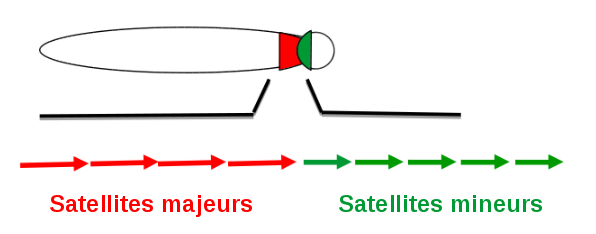
\includegraphics[scale=0.6]{tandem.png}
\scaption{Organisation schématique des chromosomes de souris : le centromère représenté est situé à une extrémité télomérique (à droite sur le schéma). En rouge, les satellites majeurs situés dans la région péricentromérique. En vert, les satellites mineurs situés au niveau du centromère.}
\label{tandem}
\end{figure}

\newpage
Les éléments répétés constituent au moins 50\% du génome de la souris. 
96\% de ces éléments sont des rétrotransposons \cite{transposables} que l'on classe en trois grandes familles selon leur mécanisme de transposition : les SINEs (short interpersed nuclear elements), les LINEs (long interpersed nuclear elements) et les ERVs (endogenous retrovirus). A eux seuls les LINE-1 représentent plus d'un tiers de la taille du génome de la souris \cite{pmid23945931}. Très abondants, ils jouent un rôle dans la structure et la fonction génomique.


\section{La marque H3K9me3}

L'hétérochromatine péricentromérique est caractérisée par plusieurs marques épigénétiques dont la triméthylation de la lysine 9 sur l'histone H3 (H3K9me3). H3K9me3 permet de fixer la protéine de l'hétérochromatine 1 (HP1) qui est ensuite capable de recruter d'autres protéines (dont SUV39H1) qui vont modifier les histones pour  étendre la région d'hétérochromatine et réprimer l'expression des gènes (Figure \ref{H3K9me3}). Cette marque contribue donc, en inhibant leur transcription, à la régulation des gènes. 
\newline H3K9me3 est essentiellement présente dans les péricentromères et les télomères (hétérochromatine constitutive) mais elle constitue également l'hétérochromatine facultative qui correspond à un état réversible, dépendant du stade de développement ou du type cellulaire. L'hétérochromatine facultative est enrichie en séquences LINES, alors que l'hétérochromatine constitutive est composée de répétition de type ADN satellite.


\begin{figure}[!h]
\centering
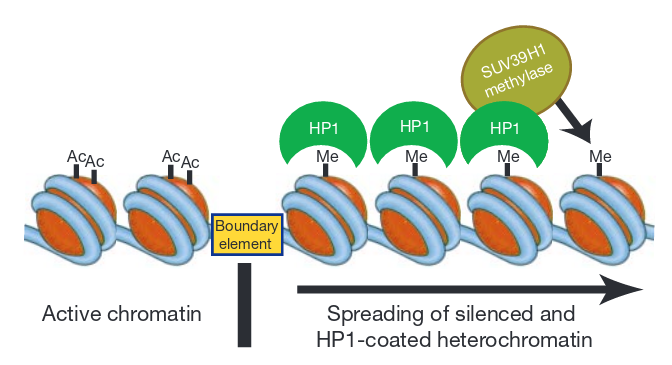
\includegraphics[scale=0.6]{H3K9me3.png}
\scaption{La marque H3K9me3 d'après \cite{intro} . Me = H3K9me3, Ac = acétylation}
\label{H3K9me3}
\end{figure}
\section{Modification épigénétique de H3K9me3}
L'équipe s'intéresse aux liens étroits qui existent entre les séquences répétées et l'organisation de la chromatine assemblée autour de ces séquences. Afin de mieux comprendre le rôle de cette chromatine sur les fonctions du centromère mais aussi sur la régulation du génome, elle s'est intéressée plus particulièrement à la marque H3K9me3, très présente dans les régions péricentromériques.
\newline Pour cela,  un modèle murin sur une lignée de souris NIH-3T3, une lignée de fibroblastes embryonnaires cultivés \textit{in vitro}, a été développé au laboratoire. 
Ce modèle vise à modifier l'hétérochromatine dans les régions péricentromériques grâce à l'utilisation d'une protéine TALE (transcription activator-like effectors) à laquelle est fusionnée un remodeleur de la chromatine (une histone lysine déméthylase). 

Les TALEs sont des protéines issues de bactéries qui possèdent un domaine de liaison à l'ADN composé de motifs répétés de 34 acides aminés. Les acides aminés 12 et 13 de chaque motif sont modulables et permettent de reconnaître une base spécifique de l'ADN selon un code (Figure \ref{construction}) \cite{TALE1}, \cite{TALE2}.
Dans notre cas, la protéine TALE a été conçue dans notre laboratoire pour pouvoir se fixer spécifiquement sur une séquence de 18 pb située dans les satellites majeurs des chromosomes.

\begin{figure}[!ht]
\centering
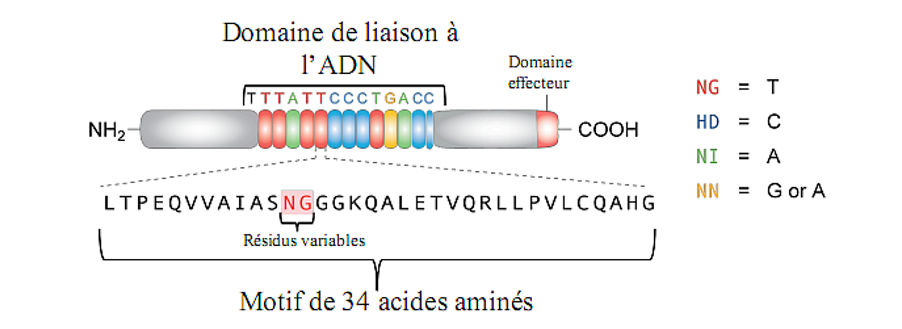
\includegraphics[scale=0.55]{domainTale.png}
\scaption{Représentation de l'organisation de la protéine TALE au niveau du domaine de liaison à l'ADN. La séquence en acides aminés d'un motif est représentée sous la TALE avec les deux acides aminés hypervariables en rouge.
A droite, les codes des acides aminés hypervariables.}
\label{construction}
\end{figure}


Deux constructions utilisant la TALE ont été réalisées : 
\begin{itemize}
 \item TALE-HD-GFP (= condition traitée): Une histone déméthylase est fusionnée à la TALE de manière à obtenir une déméthylation de H3K9me3 en H3K9me  au niveau des péricentromères.
  \item TALE-HDmutée-GFP (= condition contrôle): L'histone déméthylase a été mutée pour la rendre inactive. Cette TALE sert de contrôle car permet de garder la forme triméthylée  de H3K9 dans les régions péricentromériques.
\end{itemize}

La GFP a été fusionnée à l'extrémité C-terminale de chacune des TALEs afin de trier les cellules qui expriment la TALE à l'aide d'un facs trieur. 
 
\bigskip
Les régions péricentromériques des chromosomes de souris forment des structures particulières, puisqu’elles s’assemblent en interphase pour former les chromocentres, régions d’hétérochromatine, bien visibles après un marquage au Hoechst. L'analyse en immunofluorescence d'un grand nombre de noyaux en interphase a permis de montrer qu'il existe 2 catégories de phénotypes dans les cellules transfectées avec la TALE-déméthylase : un phénotype où la marque H3K9me3 est encore bien visible en microscopie dans les foyers de chromocentres même si une légère baisse du marquage H3K9me3 est mesurée (-16\%) et un phénotype où la diminution est très prononcée (-66\%) (Figure \ref{Résultats}A). La quantification du signal TALE dans les chromocentres montre que les cellules qui ont une forte diminution de la marque H3K9me3 sont celles qui expriment le plus la TALE-HD (Figure \ref{Résultats}B). Ces résultats indiquent que la TALE-HD est capable de se fixer spécifiquement sur les satellites majeurs  et que cette fixation est associée à une déméthylation de la marque H3K9me3 qui est proportionnelle à la quantité de TALE exprimée dans les cellules.


\bigskip

\begin{figure}[!ht]
\centering 
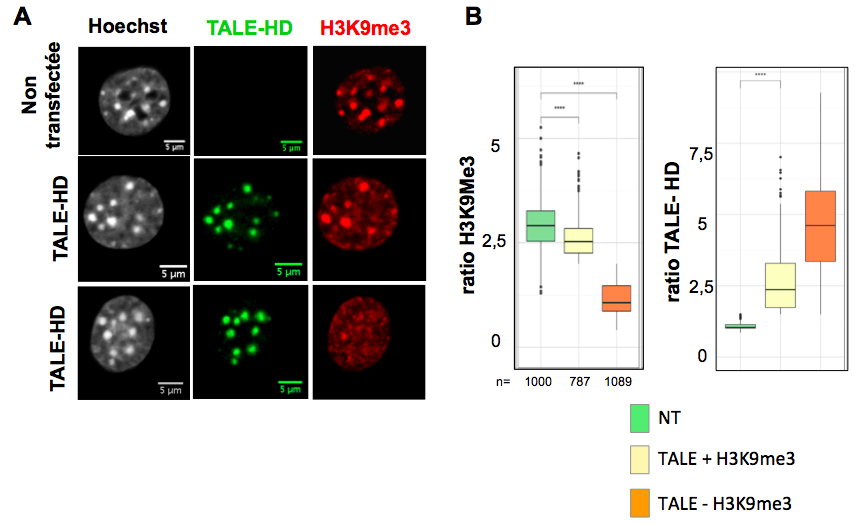
\includegraphics[scale=0.45]{result0.png}
\scaption{ A. Marquage par immunofluorescence de cellules NIH-3T3 en interphase. La TALE-HD est révélée grâce à un anticorps anti-HA (vert), H3K9me3 est révélé par un anticorps spécifique (rouge) et l’ADN est coloré au Hoechst (gris). B. Quantification du signal H3K9me3 et du signal TALE-déméthylase au niveau des chromocentres dans les cellules non transfectées (NT) et dans chacune des 2 catégories de cellules transfectées avec la TALE-HD (en jaune cellules avec présence de H3K9me3, en orange cellules sans marquage H3K9me3). n = nombre de noyaux analysés.
 (réalisé par F.Loll).}
\label{Résultats}
\end{figure}

Par ailleurs, l'équipe a pu mettre en évidence un phénotype particulier visible sur les chromosomes étalés en métaphase. Ce phénotype est présent uniquement dans les cellules exprimant la TALE-déméthylase et est associé à une forte expression de la TALE (soit 43\% des métaphases exprimant la TALE-HD).
Sur des étalements de chromosomes en métaphase, dans les cellules non transfectées, le marquage en immunofluorescence de H3K9me3 révèle un marquage majoritairement visible dans les régions centromériques et parfois aux télomères (Figure \ref{Résultats2}A). Les cellules transfectées avec la TALE-déméthylase présentent un pattern très particulier : la diminution de la marque H3K9me3 dans les régions centromériques s’accompagne d’un marquage de H3K9me3 beaucoup plus diffus s’étalant le long des bras des chromosomes, suggérant un redéploiement de H3K9me3 sur tous les chromosomes (Figure \ref{Résultats2}B).
En effet, si l'on compare les marquages illustrés dans les deux zooms (Figure \ref{Résultats2}B), à l'endroit où la TALE est recrutée (en vert), il n'y a plus d'H3K9me3 (en rose), mais ce dernier s'est déplacé sur les bras chromosomiques.
 Cette observation, tout à fait novatrice, suggère une redistribution de la marque en dehors des régions péricentromériques quand le péricentromère est déplété en H3K9me3.

\begin{figure}[!ht]
\centering 
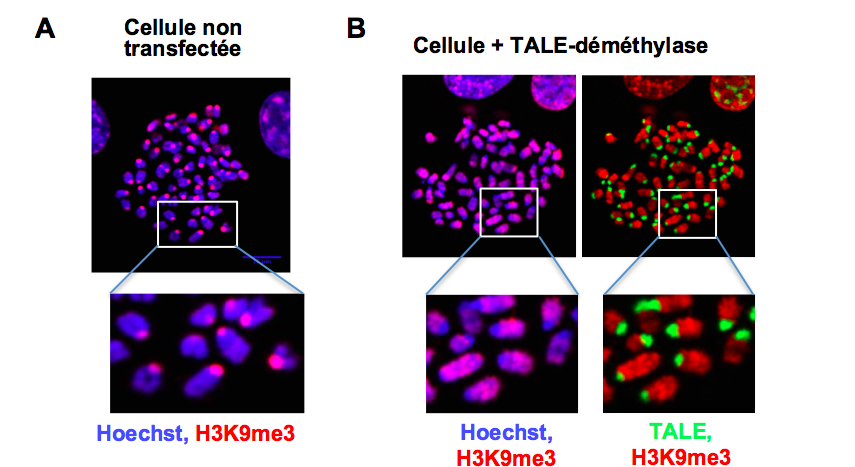
\includegraphics[scale=0.45]{result.png}
\scaption{ Etalement en métaphase des chromosomes d’une cellule NIH-3T3 non transfectée (A) ou transfectée avec la TALE-déméthylase (B). La marque H3K9me3 est révélée par un anticorps spécifique (rouge) et la TALE-déméthylase par un anticorps anti-HA (vert). L’ADN est coloré au Hoechst (bleu). La perte du marquage H3K9me3 à l’emplacement de la TALE-déméthylase est bien visible dans le zoom du milieu. (réalisé par F.Loll).}
\label{Résultats2}
\end{figure}


\newpage
Le laboratoire souhaite à présent confirmer ce résultat par une méthode à plus forte résolution : un séquençage en ChIP-Seq.
Le ChIP-Seq ou immunoprécipitation de la chromatine suivi d'un séquençage des fragments d'ADN est une technologie permettant de visualiser à l'échelle du génome les interactions entre les protéines et l'ADN. Expérimentalement, les protéines sont fixées de façon covalente à l'ADN qui est ensuite fragmenté. Puis, la marque H3K9me3 est immunoprécipitée par un anticorps spécifique. Enfin, les protéines sont dégradées, l'ADN est purifié et séquencé.
La technologie de séquençage qui a été utilisée par la plateforme de séquençage de l'Institut Curie est Illumina HiSeq \cite{pmid19997069} et 
le séquençage en paired-end de 100 pb, ce qui implique que les deux extrémités des fragments d'ADN sont séquencés  sur 100 pb chacun.
\newline 4 ChIP-Seq ont été réalisés par le laboratoire : 2 réplicats biologiques sur des cellules transfectées avec la TALE-HD  et 2 réplicats sur des cellules transfectées avec la TALE-HDm afin de cartographier la répartition de H3K9me3 à l'échelle du génome entier.
Un Input correspondant à de la chromatine non immunoprécipitée a également été séquencé afin de pallier les biais possibles de séquençage au cours de l'analyse.
\section{Objectifs du stage}
\bigskip
Dans ce contexte, mon stage a pour objectif de développer un protocole d'analyse des données de séquençage issues du ChIP-Seq et de localiser la redistribution de H3K9me3 si elle existe.
\newline
Comme H3K9me3 est une marque d'hétérochromatine, il est possible qu'elle se redistibue à la fois sur des régions répétées et sur des régions uniques. 
\newline Afin d'aborder ce projet, je vais développer les différentes stratégies que j'ai mises en place pendant ce stage. Je parlerai de l'analyse des régions uniques pour déterminer s'il existe ou non une redistribution sur les gènes ou les régions intergéniques et terminerai l'analyse par l'étude des régions répétées.



\chapter*{{
\vspace*{-2cm}}Matériel et méthodes}

\setcounter{section}{0}
\addcontentsline{toc}{chapter}{Matériels et méthodes}

  
    \section{Récupération des librairies et contrôle qualité}
    
    Les données ont été obtenues par immunoprécipitation de  la marque H3K9me3 dans des cellules de souris NIH-3T3. Les fragments d'ADN ont été isolés, purifiés puis séquencés par la technologie Illumina HiSeq 2000 à l'Institut Curie. Le séquençage a été réalisé en paired-end et génère des fragments de 2*100 paires de bases.
5 librairies ont été séquencées : un Input correspondant à de la chromatine non immunoprécipitée, deux réplicats qui ont été transfectés par la TALE-HD nommés HD1 et HD2 ainsi que deux réplicats  transfectés par la TALE-HD mutée correspondant à notre contrôle nommés HDm1 et HDm2. Les librairies ont été récupérées au format fastq.
%\newline De manière à pouvoir confirmer que la présence de la TALE ne perturbe pas le signal ``normal'' de H3K9me3, on travaille également avec des données publiques. La technologie de séquençage ainsi que la marque immunoprécipitée sont les mêmes que pour nos librairies, seules les cellules sont différentes (CD8+T : une lignée cellulaire de lymphocytes). Le séquençage est également en paired-end et les fragments générées sont de 2*150 paires de bases. Ces données ont été récupérées sur la banque de données SRA (Sequence Read Archive) du NCBI avec les identifiants suivants : SRR6228881 et SRR6228882. 

\bigskip
Une fois les différentes librairies récupérées, l’analyse qualité des séquences a été réalisée avec le programme FastQC \cite{fastqc} (version 0.11.7). 
Pour les librairies, les cinq premières paires de bases  ont été retirées de manière à améliorer la qualité globale de nos séquences. Cette étape a été réalisée grâce à FASTX Toolkit (http://hannonlab.cshl.edu/fastx\_toolkit/ ; version 0.0.14).
    
    
    \section{Alignement sur génome de référence}
    
    La détermination du génome de référence (cf Résultats, contrôle qualité et choix du génome de référence) a été réalisée en utilisant bowtie2 \cite{bowtie}(version 2.2.4) avec les paramètres par défaut sur l'Input. 
    
    Le génome de référence mm10 au format fasta et sous la forme \textit{primary assembly} a été récupéré sur Ensembl. L'indexation de ce génome a été réalisée avec le logiciel bowtie2 (bowtie2-build).
    Ensuite, nos librairies et les librairies publiques ont été alignées avec l'index construit en autorisant au maximum 2 hits multiples (paramètre -k 2) afin de différencier les régions uniques des régions multiples.

  
     \section{Détection de pics}
Deux détecteurs de pics ont été utilisés pour mettre en évidence les régions marquées par l'expérience. Nous avons tout d'abord utilisé  MACS2 \cite{MACS} (version 2.1.1.20160309)  avec les paramètres : -bampe -broad puis EPIC \cite{SICER} (version 0.2.9) avec comme paramètres des tailles de fenêtres de 20 kb et en ne conservant que les pics ayant un FDR inférieur à 1e-20.
\newline
Des diagrammes de Venn ont permis de comparer les pics des différentes conditions entre eux. Ces diagrammes ont été obtenus avec Venny \cite{Venn}.
Le package R ggplot2 a également permis de représenter les différentes tailles de pics pour chacun des échantillons.
    

   \section{Analyses spécifiques des régions uniques}
   \subsection{Traitements post-alignements et post-détection de pics}
       Pour l'étude des régions uniques, des filtres ont été effectués en sortie d'alignement. Ainsi, les samtools (version 1.3.1) ont été utilisés pour manipuler les fichiers de sortie :


\begin{itemize}
\item Elimination des reads non concordants en gardant les reads qui possèdent le flag 0x2 (-f 0x2)
\item Retrait des biais de PCR avec rmdup option -S
\item Retrait des hits multiples  : on enlève tous les reads qui ont le tag ``XS:''  car ce flag est une caractéristique des reads qui s'alignent à plusieurs endroits sur le génome
\end{itemize}

\bigskip
Le nombre de lectures dans chacune des librairies après application des différents filtres a été calculé en utilisant les samtools : samtools view -F 0x904 file | sort | uniq | wc -l. 
\newline Le flag -F 0x904 permet de retirer les reads non alignés et ceux qui ont des alignements secondaires. 
\newline
Les traitements post-alignement ainsi que la détection de pics ont été automatisés et peuvent être relancés avec le script "strategie1.sh".

\bigskip
Des Manhattan plot ont été tracés avec le package R qqman pour pouvoir filtrer les pics selon leurs FDR.
Ensuite, les pics des réplicats contrôles ont été mis en commun en utilisant l'outils bedtools \textit{merge} \cite{bedtools} (version 2.26.0).
 \newline Une fois les pics entre les réplicats mis en commun, les pics des conditions contrôles et traitées sont ensuite comparés pour récupérer les régions strictes de chevauchement (avec l'outil bedtools \textit{intersect} \cite{bedtools}, version 2.26.0) : on peut ainsi en déduire la taille exacte du génome marquée dans chacune des conditions.
      
      \subsection{Annotation des pics sur les gènes}
Avant d'annoter les pics sur les gènes, il faut différencier les régions marquées en communs ou non par nos deux conditions. 
Pour cela,  j'ai écrit un script (compare\_peak.py) pour  différencier les pics. Ce script prend en entrée deux fichiers de pics et produit 4 fichiers de sortie différents : un fichier contenant l'ensemble des pics mergés entres les deux fichiers de pics, un fichier de pics uniques au premier fichier de pics, un fichier de pics uniques au deuxième fichier de pics ainsi qu'un fichier de pics chevauchants entre les deux fichiers de pics.
 La stratégie qui a été adoptée est la suivante : 
si les pics comparés sont chevauchants, ils sont alors marqués comme communs aux deux conditions et le chevauchement le plus grand sera retenu.
Si les pics comparés ne sont présents que dans l'un des réplicats (ils sont uniques), les coordonnées de ce pics seront retenues.
Ainsi, sont extraits les  pics uniques à la condition TALE-HD ,  les pics uniques à la condition TALE-HD-mutée et les pics communs aux deux conditions.

\bigskip
      Une adaptation d'un script fourni par Madame Evelyne Duvernois-Berthet a permis d'annoter les pics avec une annotation de gènes. Cette annotation a été récupérée sur Ensembl  au format gff version GRCm38.33.
      Ainsi, on détermine si un pic est inclus dans un gène, si un gène est inclus dans un pic ou s'il y a un chevauchement entre un pic et un gène.
         Pour les gènes détectés, les voies métaboliques et ontologies GO associées ont été explorées avec DAVID \cite{GO}.
      
      \subsection{Analyse des régions uniques sur génome découpé en fenêtres}
      L'outil  bedtools \textit{makewindows} \cite{bedtools} a permis de découper le génome en 50 000 fenêtres de 55 kb (options -g -w 55000).
      Ensuite, le nombre de reads par fenêtres a été compté en utilisant les bedtools \textit{coverage} (version 2.26.0).
      Enfin, une ACP (Analyse en Composante Principale) a été tracée pour expliquer la variabilité entre tous les échantillons.
\newline Ces étapes peuvent être retrouvées dans le script "decoupage.sh".


    \section{Analyses spécifiques des éléments répétées }
    \subsection{Alignement contre une base de données d'éléments répétés (RepBase)}
 
    Afin d'avoir une estimation plus proche de la réalité du nombre de reads qui s'alignent sur les répétitions, les séquences ont été alignées contre les éléments répétés de la classe '\textit{rodrep rodent}' de la base de données RepBase \cite{repbase}.
    \newline Les séquences ont été alignées en utilisant bowtie2 \cite{bowtie}(version 2.2.4) en single end sur les mates R1 et R2 séparément, préalablement coupés pour obtenir des fragments de 35 nt. Bowtie2 a été lancé en very-sensitive.
    En sortie d'alignement, le nombre de reads s'alignant sur chacune des répétitions a été calculé.
    
    \subsection{Utilisation de RepEnrich2}
    L'outil RepEnrich2 \cite{pmid25012247} a été utilisé pour quantifier le nombre de reads qui s'alignent sur chacune des répétitions. Pour cela, le protocole disponible sur github \cite{protocole} a été appliqué.
    %(\cite{protocole}) a été suivi. : 
    Dans cet outil, les reads sont dans un premier temps alignés de manière unique avec bowtie2 (option -k 1) sur le génome mm10. Les reads uniques et multiples sont séparés et les reads multiples sont assignés à un fichier FASTQ.
    En parallèle, l'annotation des répétitions est réalisée à partir des annotations d'éléments répétés de repeatMasker (Repeatmasker.org). 
    Le chevauchement des reads uniques avec des éléments répétés est testé. Les reads multiples sont alignés contre l'assemblage des répétitions en utilisant bowtie2.
    Enfin, le nombre de reads s'alignant contre les familles d'éléments répétés ou les classes d'éléments répétés est déterminé. Ainsi, pour chaque élément répété, RepEnrich2 fourni un comptage de reads.
 %   \newline Les comptages générés par RepEnrich2 ont été analysés par analyse différentielle en utilisant le package R DESeq2 \cite{deseq} (normalise et recherche des répétitions différentiellement exprimées en se basant sur un modèle de binomiale négative)
 \newline
 L'utilisation de RepEnrich2 a été automatisée et peut être lancée avec le script "RepEnrich.sh".
 Le script R d'analyse des résultats est "repenrich.R".
 
    

    \subsection{Réalisation des MAplot}
    Les MAplot correspondent à la représentation des Log2FC en fonction de la moyenne des comptages normalisés.
Seule la librairie HD2 pour la condition traitée et les librairies HDm1 et HDm2 pour la condition contrôle ont été prises en compte pour les calculs.
   Le Log2FC calculé correspond au rapport de la librairie HD2 normalisée sur la moyenne des librairie HDm normalisées 
(
 $log2((\frac{HD2}{Taille librairie}$ / 0.5* ($\frac{HDm1}{Taille librairie}$+$\frac{HDm2}{Taille librairie}$)) ).     
 \newline
Le Log2 de la moyenne des comptages correspond à la moyenne des comptages de HD2 et de HDm ($log2(\frac{HD2+HDm}{2}$)).
          
          
    \section{Analyse du signal}

         \subsection{Normalisation du signal}      
         Deux types de normalisations ont été réalisées : 
         \begin{itemize}
         \item Pour visualiser le signal global sur le génome de référence : le signal de chaque librairie a été normalisé en utilisant bamCompare de l'outil deeptools \cite{deeptools} (version 3.0.2). 
      Les librairies ont été normalisées par soustraction de l'Input à l'IP en utilisant l'option ``substract bins 10''.
    \newline
      Ainsi, un signal  plus important dans l'IP que dans l'Input se traduira par un résultat positif et inversement un signal plus important dans l'Input que dans l'IP par un résultat négatif.
      Pour utiliser bamCompare, il faut fournir les fichiers d'alignement ainsi que l'indexation de ces fichiers. L'indexation a été réalisée par les samtools.
      \item Pour visualiser une région spécifique du génome (par exemple les satellites majeurs appelés GSAT) : le signal de chaque librairie a été normalisé uniquement par la taille des librairies en utilisant bamCoverage de l'outil deeptools (version 3.0.2).
       \end{itemize}
       
    \subsection{Visualisation du signal}
      Les différents alignements et pics obtenus ont été visualisés avec le logiciel IGV (Integrative Genomics Viewer \cite{IGV} : version 2.4.8).
       L'annotation des répétitions et des gènes a été obtenue sur l'UCSC (Clade mamals, genome mouse, assembly mm10, group Genes and Genes prediction, track UCSC genes et table kgXref) au format gff et a été utilisée pour visualiser les reads sur les éléments répétés. 
      Pour la suite du manuscrit, le code couleur est le suivant : bleu pour les librairies contrôles (HDm1 et HDm2), vert pour la librairie publique, rouge pour HD2 et orange pour HD1.
      
\bigskip
      La représentation en circos \cite{circos} (version 0.69-6) a été utilisée pour apporter une vue d'ensemble de la répartition du signal sur le génome. Le signal normalisé IP-Input est représenté selon le code couleur présenté ci-dessus en utilisant l'échelle [10:100]. Les pics EPIC de chaque librairie sont indiqués sous chaque signal leur correspondant.
      
     

\section{Analyse en composante principale (ACP)}
     
     Pour décrire les jeux de données des ACP ont été réalisées grâce au package FactoMineR \cite{ACParticle} avec l'option ``scale.unit=TRUE'' pour centrer et réduire.
  

\section{Mise à disposition des scripts}
Les scripts utilisés pendant le stage sont disponibles à l'adresse suivante : https://github.com/MathildeBertrand/STAGE\_M2.git
\newpage
\chapter*{{
\vspace*{-2cm}}Résultats}
\setcounter{section}{0}
\addcontentsline{toc}{chapter}{Résultats}
   

    \section{Développement d'un protocole d'analyse pour la marque H3K9me3}
        
   L'analyse classique des données de ChIP-Seq consiste à vérifier la qualité des librairies, localiser les reads sur un génome de référence (étape de mapping avec bowtie2), détecter les régions statistiquement enrichies par l'expérience (étape de détection de pics) et à analyser ces régions.
  % Cette analyse a été réalisée. A l'issue de l'analyse qualité, les séquences ont été ``trimmées''  pour en améliorer la qualité globale.
   \newline
   Ce protocole standard pose problème dès qu'il s'agit d'analyser la présence d'une marque chromatinienne spécifique de l'hétérochromatine qui est par conséquent essentiellement présente sur des éléments répétés.
   Ainsi, nous avons imaginé un protocole permettant de séparer l'analyse des régions uniques du génome, en particulier  les gènes, et l'analyse des régions répétées (centromères, télomères et éléments transposables principalement) (Figure \ref{Résultats expérimentaux}).
   \newline
   Pour l'étude des régions uniques, le retrait des reads non concordants, des biais de PCR et des hits multiples a permis de supprimer la redondance de nos librairies. La détection de pics a ensuite été réalisée sur les reads uniques en utilisant l'Input comme donnée de normalisation.
   \newline
  Pour l'étude des régions répétées, deux stratégies ont été testées en parallèle.
  \newline D'abord, un alignement des reads sur une base de données d'éléments répétés (RepBase \cite{repbase}) dans le but de déterminer les répétitions les plus enrichies.
  Ensuite, un outil dédiée (RepEnrich2 \cite{pmid25012247}) à l'analyse des éléments répétés a été utilisé pour quantifier le nombre de reads sur chacun des éléments répétés.

\begin{figure}[!ht]
\centering
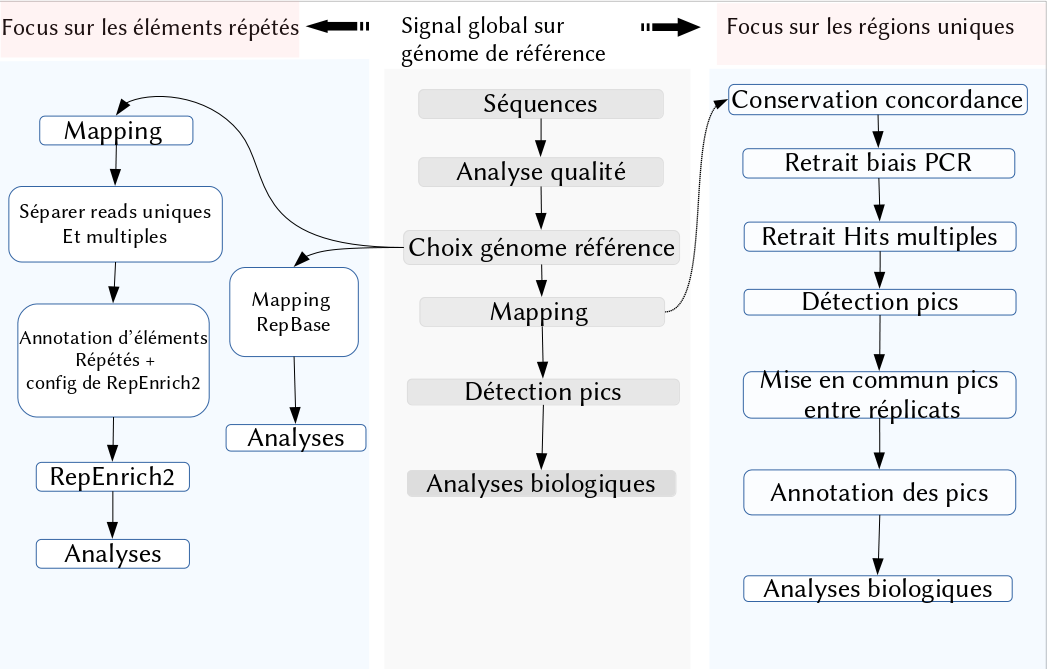
\includegraphics[scale=0.53]{pipeline.png}
\scaption{ Mise en place du protocole d'analyse. A gauche : focus sur les éléments répétés. A droite : focus dans les régions uniques. Au centre : analyse du signal global sur le génome de référence.}
\label{Résultats expérimentaux} 
\end{figure}
%\begin{landscape}
%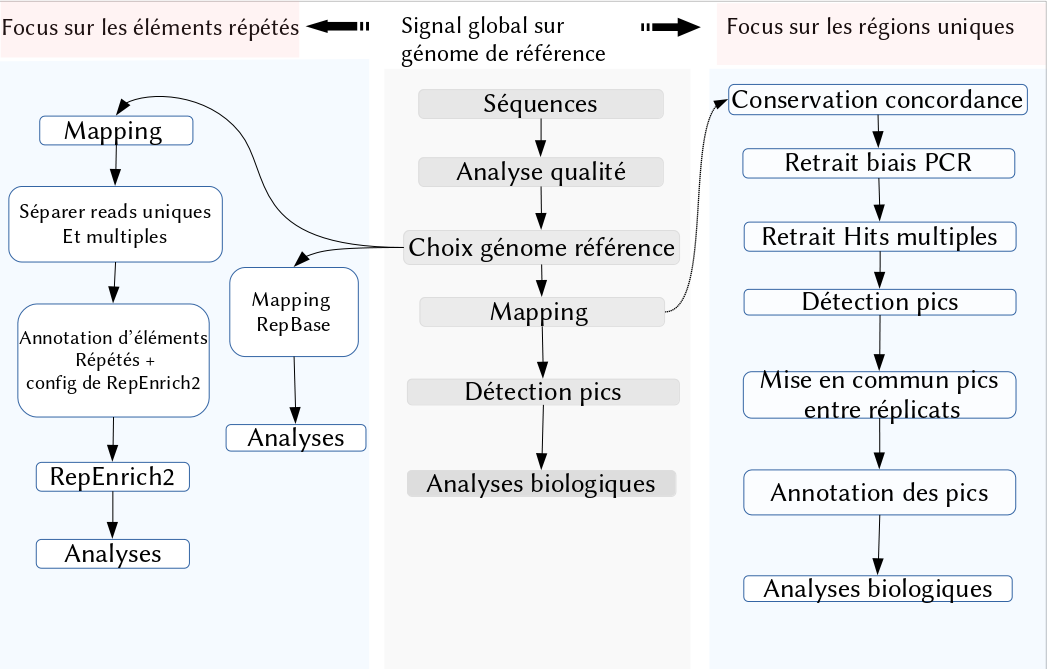
\includegraphics[scale=0.65]{pipeline.png}
%\end{landscape}
\newpage
    \section{Contrôle qualité et choix du génome de référence}\label{Test}
    Le nombre de lectures varie entre 2x30 et 2x55 millions pour nos librairies  (Table \ref{tab1}). 
 \begin{center}
 \begin{tabular}{|p{4cm}|p{2cm}|p{2cm}|p{2cm}|p{2cm}|p{2cm}|}
\hline
  & Input &HD1 & HD2 &  HDm1 & HDm2 \\
\hline
Nombre de reads par mates (millions) & 52 &  29 & 55 & 33 & 38   \\
\hline
\end{tabular}
\captionof{table}{Table du nombre de lectures obtenues pour chacune des librairies (en millions de reads)}
\label{tab1}
\end{center}

La qualité des séquences est évaluée, entre autre, par le score phred qui est un score relié de manière logarithmique à la probabilité d'erreur d'identification d'une base. Il varie entre 0 et 40. 
 Dans l'ensemble, le score par nucléotide est autour de 40.  Seul le tout début des séquences est de moins bonne qualité : les cinq premières paires de bases pour nos librairies ont un score phred autour de 32 (Figure \ref{fastqc}). Afin d'améliorer la qualité globale, ces bases ont été retirées.
    
\begin{figure}[!h]
\centering
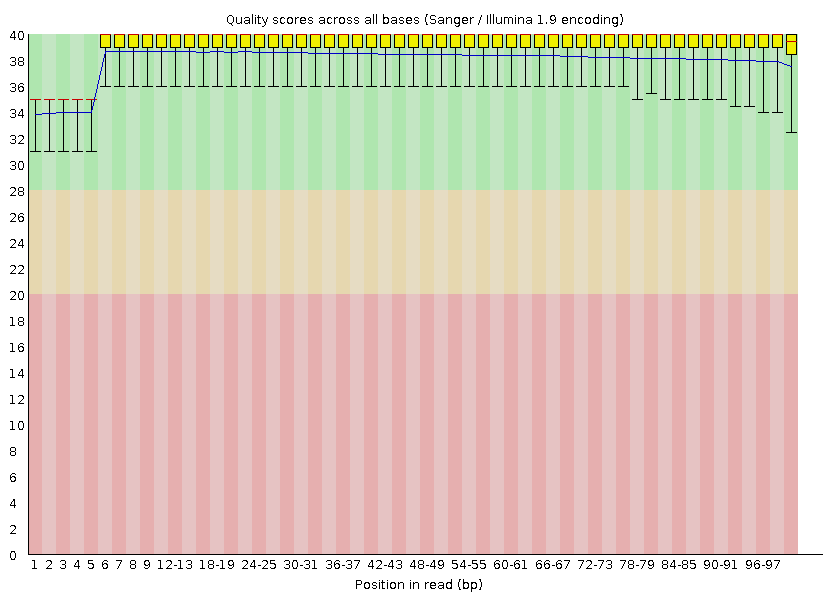
\includegraphics[scale=0.6]{fastqc.png}
\scaption{Un des graphiques de l'analyse qualité obtenu avec FastQC pour la librairie HD1-mate1 présentant par des boîtes à moustaches la qualité globale de chaque position de tous les reads. Les 5 premières paires de bases ont ensuite été retirées pour la suite de l'analyse. Les graphiques obtenus avec les autres librairies sont similaires.}
\label{fastqc}
\end{figure}

    Comme il n’existe pas de  génome de référence pour notre lignée de souris NIH-3T3, il a fallu déterminer, préalablement à l'analyse, parmi l’ensemble des génomes de référence de souris possédant une annotation dans Ensembl, celui qui était le plus proche de notre lignée. 
    Pour cela, l’Input de nos données a été aligné contre les génomes accessibles (15 au total) et celui qui avait le meilleur pourcentage d’alignement a été conservé. 
    Les pourcentages d'alignement pour les différents génomes sont similaires exceptés pour deux d'entre eux qui sont autour de 15\% (wsbeij et 129s1svimj).
    \newline Le meilleur pourcentage de mapping (98.38 \%) a été obtenu pour le génome mm10 qui a donc été sélectionné pour la suite des analyses.

    \section{Perte modérée de signal au péricentromère}
    Rappelons que l'expérience réalisée consiste à déméthyler H3K9me3 en H3K9me sur les satellites majeurs du péricentromère pour observer l'impact que cela pourrait avoir sur le génome. \\
    Afin de valider l'expérience, j'ai sélectionné, en sortie d'alignement, une des rares régions comportant un grand nombre de répétitions de satellites majeurs, s'étendant sur 40 kb sur le chromosome 9 aux positions 3000 à 3040 kb.  
    Entre 15 et 17\% de reads s'alignent en moyenne sur cette région, il s'agit de la plus grande région de satellites majeurs assemblée dans le génome mm10.
    Le signal  normalisé  par la taille de la librairie par bamCoverage a été visualisé avec IGV (Figure \ref{IGV}).
    
    \bigskip
    Le signal semble identique pour chaque librairie. On ne peut pas déterminer visuellement s'il y a eu ou non une perte de la marque H3K9me3 dans cette région.       
   \bigskip
    \begin{figure}[!h]
   \centering
    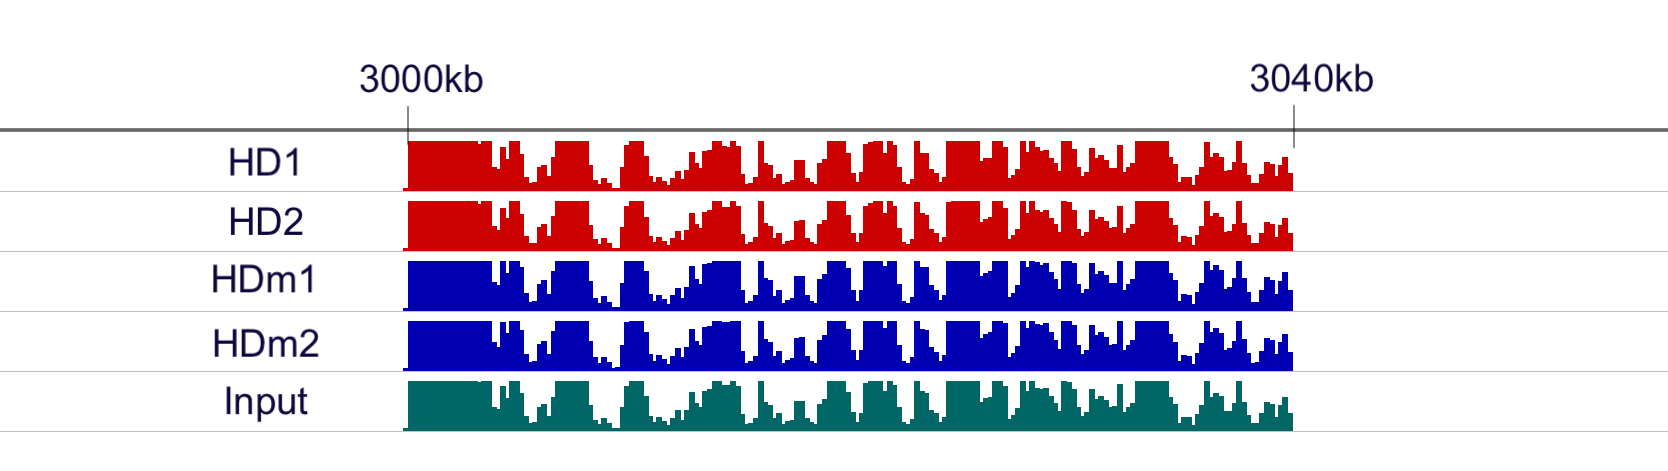
\includegraphics[scale=0.4]{GSATRPKM.png}
    \scaption{ Capture IGV d'une région de satellites majeurs de 40 kb sur le chromosome 9. Le signal est normalisé par la taille de chaque librairie.   Les réplicats traités HD1 et HD2 sont en rouge, les réplicats contrôles HDm1 et HDm2 en bleu et l'Input est en vert. L'échelle est la même pour tous les échantillons :  0 à 1200.}
  \label{IGV}
  \end{figure}

Afin d'estimer de façon plus précise l'éventuelle perte de signal H3K9me3 dans les cellules traitées avec la TALE-déméthylase dans cette région, j'ai représenté le rapport des librairies traitées par les librairies contrôles. Si ce ratio est inférieur à 1, cela signifie qu'il y a plus de signal dans la condition TALE-déméthylase mutée que dans la condition TALE-déméthylase et donc qu'il y a bien une perte de la méthylation de H3K9. 
Quand on calcule le ratio HD1 par rapport à la moyenne de HDm1 et HDm2 et celui de HD2 par rapport à la moyenne de HDm1 et HDm2, on observe le même comportement (Figure \ref{IGVratio}) :  en moyenne, le ratio est de 0.88, soit une perte de 12\%.
Il y a donc 12\% de méthylation en moins dans les réplicats HD que dans les réplicats HDm sur cette région du génome.
De plus, comme le ratio est identique entre HD1 et HD2, il semblerait que les réplicats se comportent comme des réplicats.

 \begin{figure}[!h]
   \centering
    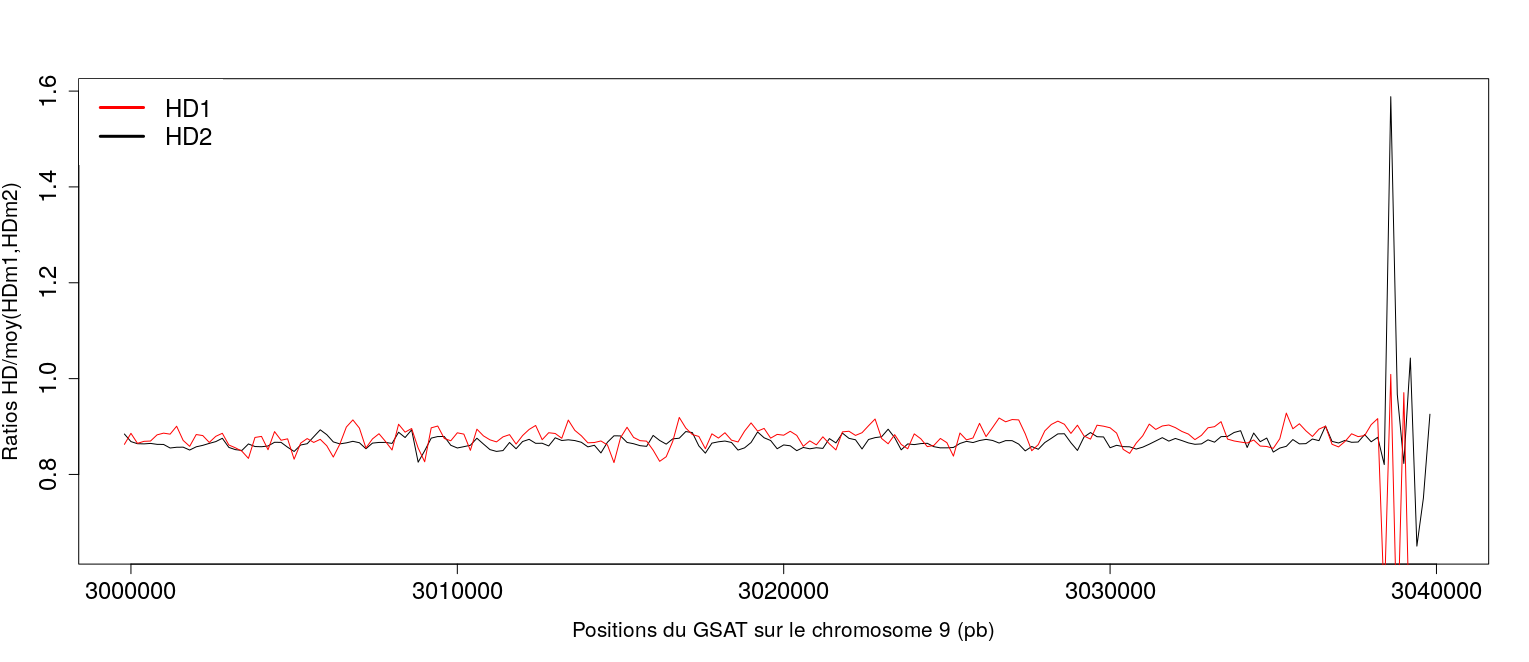
\includegraphics[scale=0.45]{Rplot200.png}
   \scaption{Quantification de la perte de  la méthylation de H3K9 dans les conditions traitées par rapport au contrôle sur la région des satellites majeurs du chromosome 9. En rouge,  HD1 et en noire HD2. }
  \label{IGVratio}
  \end{figure}
  

  D'autres régions de satellites majeurs sont présentes dans mm10.  Un comptage du nombre de reads présents sur l'ensemble des GSAT a d'ailleurs montré qu'en moyenne (Annexe, Table 4), il y a 20\% de méthylation en moins dans les réplicats HD que dans les réplicats contrôles.
Ce résultat indique que l'expression de la TALE-déméthylase dans les cellules NIH-3T3 induit une déméthylation modérée de la marque H3K9me3.
      \newpage
    \section{Une redistribution difficile à mettre en évidence sur les régions uniques}
     
      L'alignement des reads sur le génome de référence a été réalisé en autorisant au plus deux hits multiples. Ainsi, si un read s'aligne sur plusieurs positions sur le génome, seules les deux meilleures positions seront retenues. Ce paramètre d'alignement est nécessaire car il nous permet d'identifier les reads uniques et de les isoler pour chacune des librairies : ils représentent entre 62 et 65 \% de la taille des librairies. En moyenne 20  \% des reads correspondent à des hits multiples, 18  \%  à  des biais de PCR et  3\% sont non concordants (Table \ref{tab2}).
    \begin{table}[h]
  \begin{tabular}{|p{5cm}|p{2cm}|p{2cm}|p{2cm}|p{2cm}|p{2cm}|}
\hline
  & HD1 & HD2 &  HDm1&  HDm2 & Input\\
\hline
Nombre de reads initiaux & 29917010 &  55242254 & 33530582 & 38385939 & 52068315  \\
\hline
\% de reads alignés & \multicolumn{5}{c|}{98}  \\
\hline
\% de reads retirés après appariement& \multicolumn{5}{c|}{3}  \\
\hline
\% de reads retirés après suppression des biais de PCR & 17 & 16.5 & 18 & 18 & 17  \\
\hline
\% de reads retirés après suppression des hits multiples & 20 & 21 & 21 & 21 & 19  \\
\hline
\% de reads conservés & 64 & 64 & 63 & 62 & 65  \\
\hline
Nombre de reads conservés& 18741919 &34982522 & 20723260 & 23980456 & 33676826  \\
\hline
\end{tabular}

\scaption{Les différentes étapes de filtres appliqués sur chacune des 5 librairies et le nombre de reads finalement conservés à l'issu de ces étapes (le nombre de reads est en millions et doit être multiplié par 2, puisque le séquençage est en paired-end).}
\label{tab2}
\end{table}

La détection de pics permet de mettre en évidence les régions du génome qui présentent un enrichissement de la marque H3K9me3.
 Il est connu que les modifications d'histones génèrent des pics pouvant faire plusieurs centaines de kilobases.
 MACS2 a dans un premier temps été utilisé. Les pics obtenus étaient peu nombreux, petits et  la plupart n'étaient pas en adéquation avec le signal des librairies et cela, malgré l'important nombre de paramètres testés (Annexe, Figures \ref{MACS2D} et \ref{MACS2T}).
C'est pour cela que nous avons utilisé un autre détecteur de pic : EPIC. Les résultats obtenus avec EPIC sont plus cohérents avec notre signal et les pics obtenus sont plus larges, ce qui est d'autant plus cohérent avec la notion de pics larges tels que semble être le signal de H3K9me3 (Annexe Figure \ref{circosTout}).

\bigskip
5 kb, 10 kb et 20 kb sont les différentes tailles de fenêtres qui ont été testées. En faisant varier ces paramètres, les mêmes pics ont été trouvés à la différence qu'en augmentant la taille des fenêtres les petits pics sont fusionnés. Nous avons choisi de garder des fenêtres de 20 kb.
\newline
 EPIC associe à chacun des pics un FDR (False discovery Rate) correspondant à la probabilité de détecter un pic à tort sur le génome : plus le FDR est élevé, moins les pics détectés sont probables.
Pour limiter la proportion de faux pics dans notre jeu de données, la distribution du nombre de pics par chromosome selon les différentes valeurs de FDR a été tracée pour les différentes librairies (Figure \ref{HD2}, Annexe Figures \ref{HDm1M} et \ref{HDm2M}). 
En fixant ce seuil à 1e-20, nous sélectionnons un grand nombre de pics tout en limitant la détection de pics aberrants.
\begin{figure}[!h]
\centering
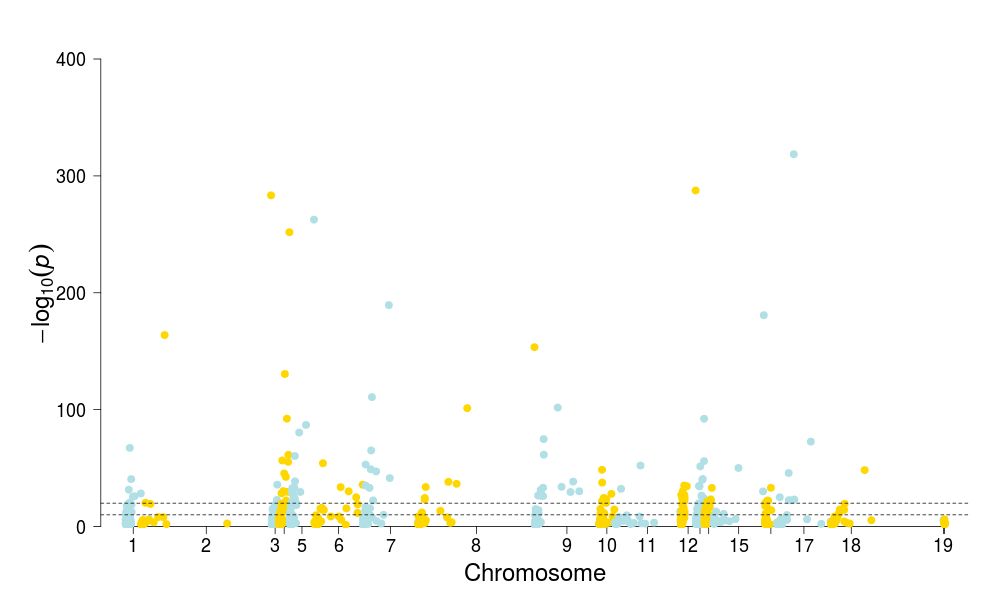
\includegraphics [scale=0.4]{manhattanPlot_lib18EPIC.png}
\scaption{Manhattan plot représentant le FDR en log10 des pics obtenus avec EPIC sur les différents chromosomes pour la librairie HD2. Deux traits horizontaux ont été tracés correspondant aux FDR à 1e-10 et 1e-20. }
\label{HD2}
\end{figure}


 \bigskip
Une fois la détection de pics réalisée, plusieurs questions se posent alors :  les pics sont-ils en adéquation avec le signal ? Où sont localisés les pics ? La localisation des pics est-elle identique entre les deux conditions ? \\
Pour y répondre, nous avons commencé par visualiser le signal et les pics sur l'ensemble du génome.
   Ainsi, en positionnant les différents chromosomes du génome mm10 de manière circulaire, le circos (Figure \ref{circoss}) permet de visualiser pour chaque librairie le signal normalisé IP-Input par bamCompare.
  \newline Nous pouvons voir que le signal est réparti sur l'ensemble du génome de référence de la même manière pour les librairies HD et les librairies HDm. Seule la hauteur du signal semble varier entre les librairies. En effet, il semble qu'il y ait plus de signal dans la librairie HD2 que dans les autres. 
   \newline  Les pics obtenus avec EPIC et filtrés à un FDR inférieur à 1e-20 sont également visualisés et correspondent sur le graphique aux rectangles. On voit ici que les pics se répartissent sur l'ensemble du génome à l'exception des chromosomes X et Y.  Les pics détectés ici ne sont pas optimaux car certaines régions ont beaucoup de signal et aucun pic associé n'est détecté. En ce qui concerne les pics, il n'est pas possible à cette résolution de déterminer si il y a ou non une modification du signal entre les conditions HD et HDm.

    \begin{figure}[!h]
    \centering
    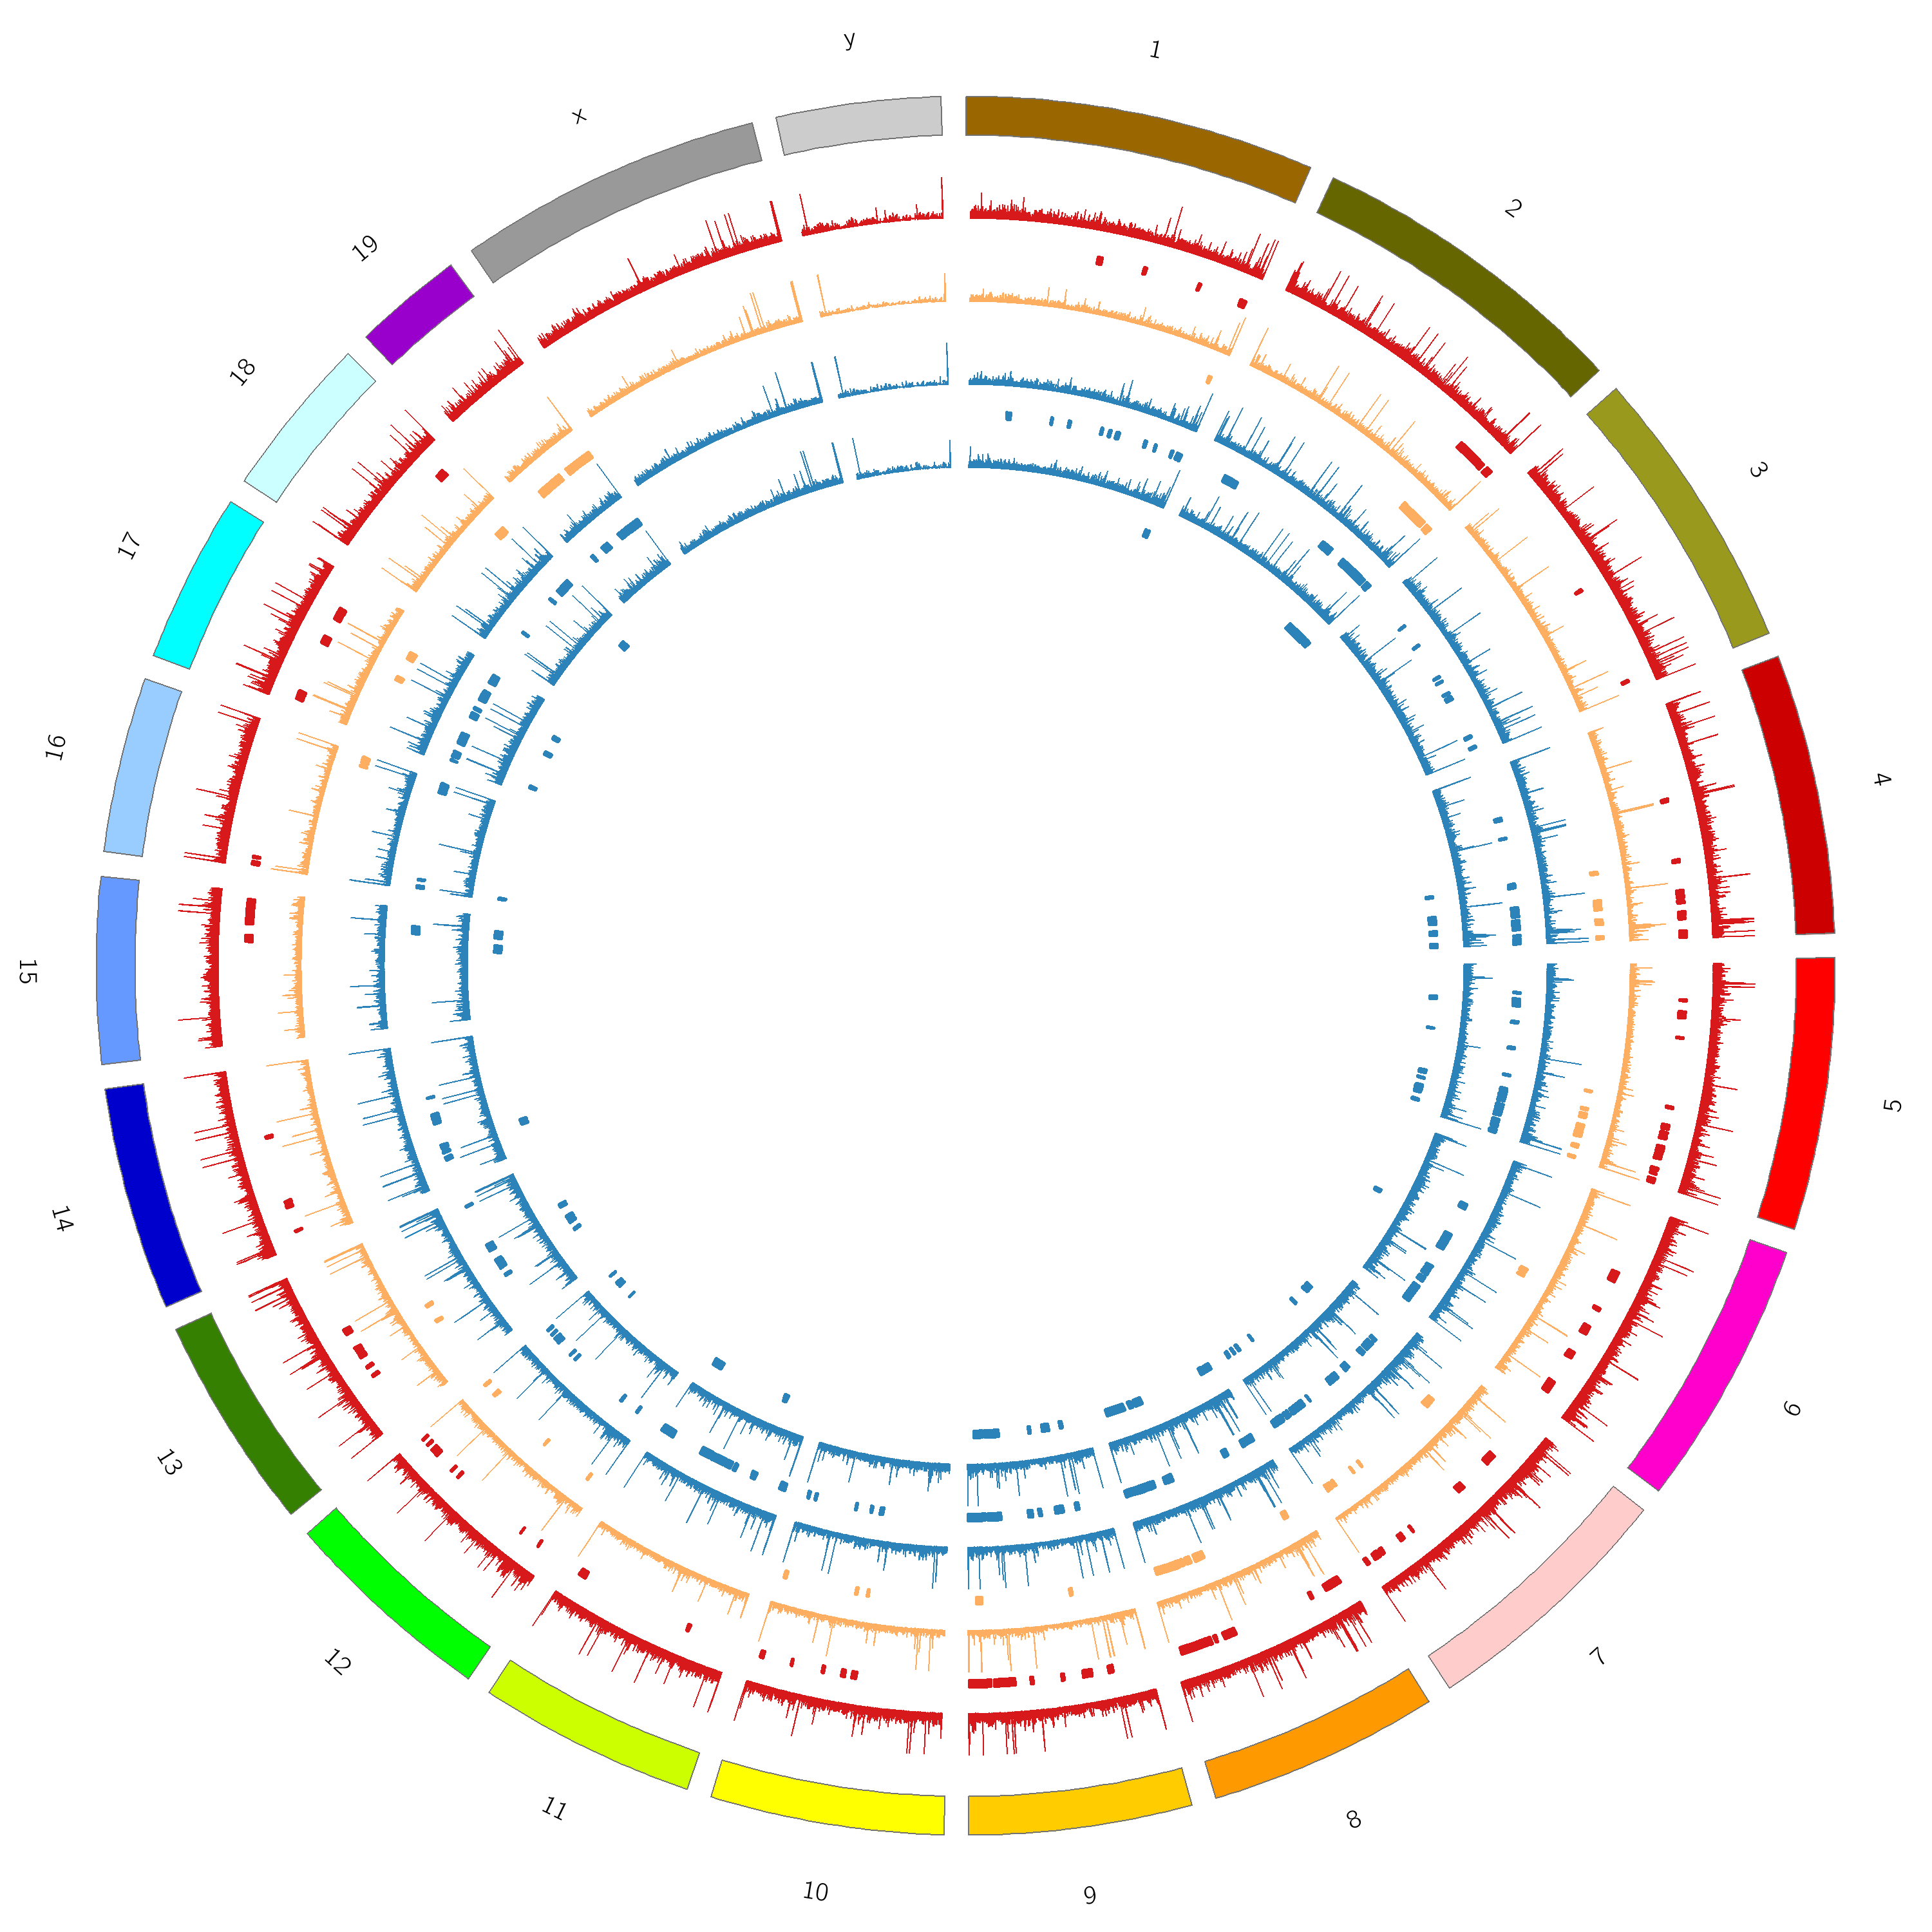
\includegraphics[scale=0.2]{circos_signal_rgunique_peaks_10-100_e20.png}
    \scaption{Répartition du signal normalisé  et des pics pour les différentes librairies.
     Le génome de référence mm10 est représenté par le cercle le plus à l'extérieur avec chaque chromosome représenté par une couleur. 
     Les autres cercles représentent les signaux normalisés (IP-Input) et les pics détectés dans les librairies. Les librairies traitées sont en orange pour HD1 et en rouge pour HD2, les librairies contrôles sont bleues, HDM2 étant la plus proche du centre.
    L'échelle est fixée arbitrairement à [10:1000]. Les pics EPIC à FDR inférieur à 1e-20 sont représentés sous le signal leur correspondant. }
    \label{circoss}
    \end{figure}
    
    \newpage
    Comme le signal normalisé IP-Input des librairies - visualisés précédemment - suggérait que la hauteur du signal de la librairie HD2 était plus forte que celle des autres librairies, nous avons voulu approfondir l'analyse du comportement des réplicats dans les régions uniques.
    Pour cela,  une analyse sur le génome découpé en fenêtres a été réalisée : le génome de 2 730 871 774 bp a été découpé en 50 000 fenêtres de 55 kb, puis le nombre de reads uniques par fenêtres a été compté. 
   Une Analyse en Composante Principale (ACP, Figure \ref{ACP1}) a ensuite été réalisée pour visualiser la variabilité globale entre les différentes librairies.
   Les dimensions 1 et 2 expliquent le mieux cette variabilité. Nous pouvons voir que la librairie HD2 se distingue des 3 autres et notamment du réplicat HD1 (96\% de la variabilité dans la dimension 1).
   \newline Quant à la librairie HD1, elle se comporte en moyenne comme les deux librairies contrôles HDm1 et HDm2.
    Ce résultat suggère que les réplicats traités ne se comportent pas comme deux réplicats et l'un d'eux (HD1) semble plus proche des 2 librairies HDm1 et HDm2 que de la librairie HD2.
     Nous avons fait le choix de la garder pour les visualisations et de la retirer pour la suite des analyses des régions uniques.
 
   \begin{figure}[!h]
    \centering
    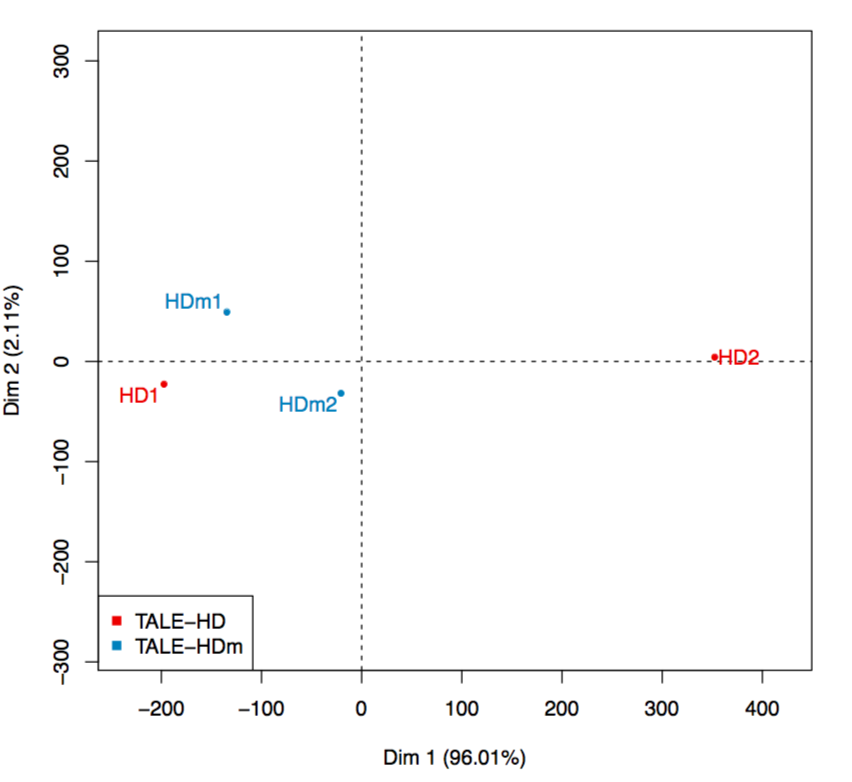
\includegraphics[scale=0.32]{ACP_uniques.png}
    \scaption{ACP réalisée à partir du nombre de reads comptés sur des fenêtres de 55 kb du génome pour les différents échantillons. Les dimensions 1 et 2 sont celles qui expliquent le mieux la variabilité des librairies. En rouge les réplicats avec la TALE-déméthylase (TALE-HD), en bleu avec la TALE-déméthylase mutée (TALE-HDm).}
    \label{ACP1}
   \end{figure}


  Comme les résultats de l'ACP suggèrent que HD1 semble se comporter comme les réplicats contrôles, nous avons émis l'hypothèse que la déméthylation de la marque H3K9me3 avait moins bien fonctionné sur ce réplicat. Nous l'avons donc écartée pour la suite des analyses.
  Nous travaillerons avec un seul réplicat traité et deux réplicats contrôles,  ce qui nous limitera à réaliser une analyse qualitative, plutôt que quantitative.
  
  Dans un premier temps, nous avons mis en commun les pics des réplicats contrôles (HDm1 et HDm2), selon le script détaillé dans le matériel et méthodes et nous les avons comparés aux pics de la librairie HD2. 
 \\ 
 La distribution de la taille des pics est présentée à l'aide de violin plot (Figure \ref{violin}).
 Les violin plot sont similaires aux boxplot à la différence qu'ils permettent de montrer la courbe de densité de probabilité des différentes valeurs.
Comme il était possible de le voir sur le circos, certains pics sont très larges et peuvent atteindre des tailles allant jusqu'à 20 Mb pour HD2 et 25 Mb pour HDm.  Dans les deux conditions, la majorité des pics sont de petite taille (autour de 100 kb) et il semblerait qu'il y ait plus de petits pics en condition HD qu'en condition HDm. En moyenne, la taille des pics est autour de 993 kb pour les deux conditions.
   
   \begin{figure}[!h]
    \centering
    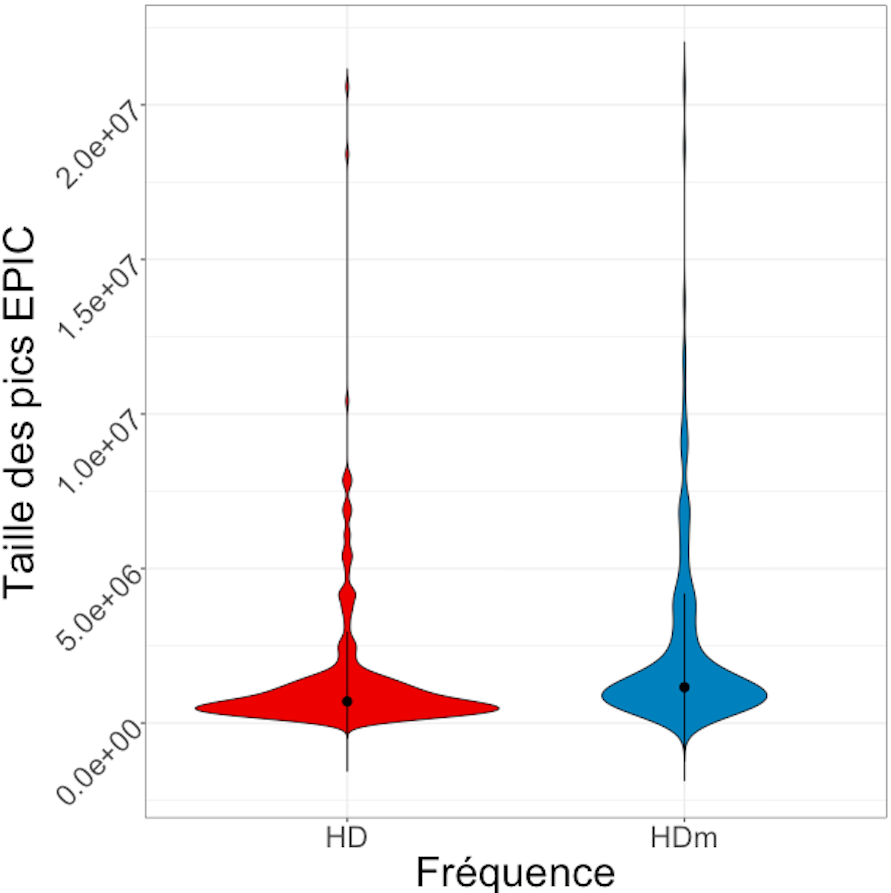
\includegraphics[scale=0.35]{violinPlot_lengthEPIC.png}
    \scaption{
    Violin plot représentant la répartition de la taille des pics en paire de bases pour la librairie HD2 (en rouge) et pour  les librairies HDm1-HDm2 en bleu. Le point noir représente la médiane.}
    \label{violin}
    \end{figure}
    

   Dans un second temps, les pics identifiés dans chacune des conditions ont été comparés.
   Les pics uniques à la condition traitée correspondent à un gain de marquage dans la condition HD par rapport à HDm, alors que les pics uniques à la condition HDm correspondent à une perte de signal dans la condition HD par rapport à HDm.
   Les pics communs sont des régions où le signal est présent dans les deux conditions  (Figure \ref{Venny}).
    \newline
    Les pics de la condition contrôle couvrent 474 Mb alors que les pics de la condition traitée couvrent 387 Mb de la taille du génome, soit 1,2 fois moins de couverture dans la condition traitée que dans la condition contrôle. La marque H3K9me3 est donc moins représentée dans les régions uniques suite à l'expression dans les cellules de la TALE-déméthylase.
De plus, nous constatons que seulement 94 Mb sont spécifiquement couvertes par des pics propres à la condition TALE-déméthylase, suggérant ainsi une faible redistribution de la marque dans les régions uniques.

\begin{figure}[!h]
\centering
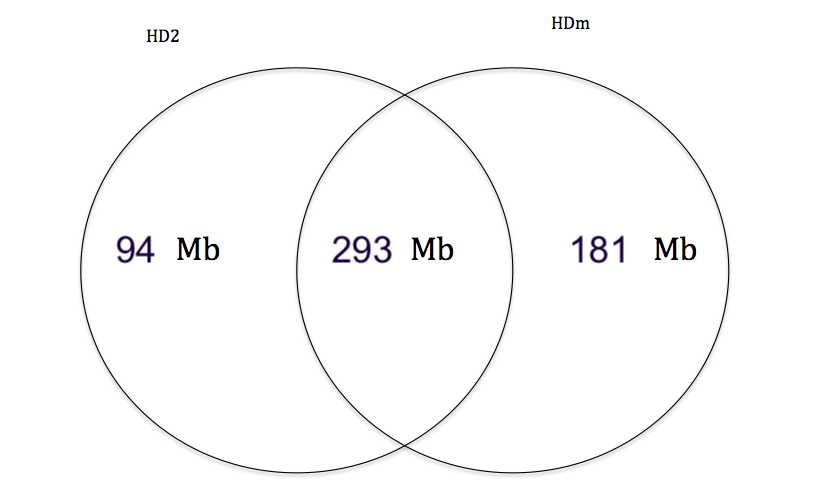
\includegraphics[scale=0.3]{Venny.png}
\scaption{Diagramme de Venn représentant le nombre de mégabases couvertes par des pics dans les régions géniques et intergéniques dans les conditions HD2 et HDm. L'annotation de ces pics sur des gènes a été réalisée. La proportion de pics sur les régions géniques et intergéniques est représentée par les piechart pour chaque condition}
\label{Venny}
\end{figure}

\newpage
Dans un troisième temps, nous avons cherché à déterminer si la redistribution modérée observée dans la condition TALE-HD est essentiellement génique, intergénique ou bien les deux.
Pour répondre à cette question, les pics ont été annotés avec une annotation de gènes et  ces gènes ont été dénombrés dans chaque condition.
\newline Quatre cas de figures peuvent être distingués. (i) le ``gain de marquage''  correspond à un gène marqué dans la condition traitée qui ne l'est pas dans la condition contrôle ;
(ii) la ``perte de marquage'' est le cas où le gène est marqué dans la condition contrôle mais ne l'est plus dans la condition traitée ; (iii)
la ``modification du signal au sein d'un gène'' correspond à un gène qui est marqué dans les deux conditions mais pas au même endroit ; (iv)
quand un gène est marqué dans les deux conditions et au même endroit, on dit qu'il n'y a ``pas de redistribution'', cependant il peut juste y avoir une modification de l'intensité du marquage.
Ces différents cas de figure sont illustrés dans la Table 3.
 


 \begin{table}[h]
  \begin{tabular}{|p{10cm}| p{5cm}|}
\hline
  Perte de marquage dans la condition HD & 
  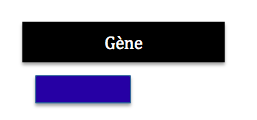
\includegraphics[scale=0.4]{perteimg}
   \\
\hline
Gain de marquage dans la condition HD &   
\includegraphics[scale=0.4]{gainimg}  \\
\hline
Redistribution au sein d'un gène &  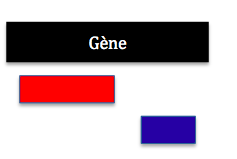
\includegraphics[scale=0.4]{Redis}\\
\hline
Pas de redistribution &  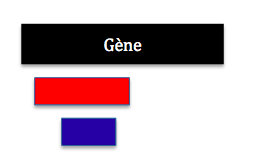
\includegraphics[scale=0.4]{NoRedis}  \\
\hline
\end{tabular}
\scaption{Représentation des différentes répartitions de pics au sein des gènes, selon la condition contrôle (pic représenté par un rectangle bleu) ou la condition TALE-HD (pic représenté par un rectangle rouge).}
\end{table}

\bigskip

La catégorie dans laquelle le plus de gènes ont été identifiés est celle de la ``perte de marquage" qui touche plus de 3596 gènes (Figure \ref{genes}). Pour un grand nombre de gènes (2244), le statut épigénétique de la marque H3K9me3 n'a pas changé : ce sont des gènes qui appartiennent à la catégorie "redistribution au sein d'un gène" ou à la catégorie "pas de redistribution".
Seuls 259 gènes sont identifiés dans la catégorie "gain de marquage". 

\begin{figure}[!h]
\centering
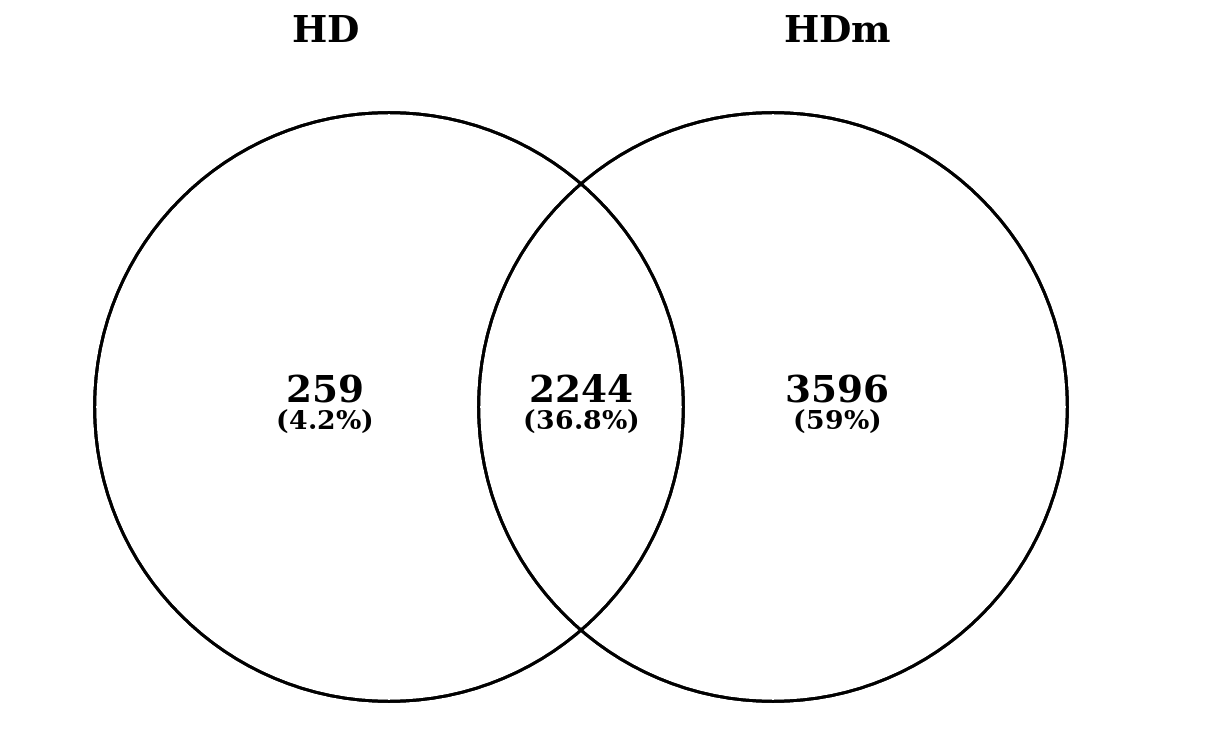
\includegraphics[scale=0.2]{VennDiag_HDvsHDm_e20.png}
\scaption{Diagramme de Venn représentant le nombre de gènes identifiés dans chacune des conditions}
\label{genes}
\end{figure}

Nous avons illustré quelques régions identifiées afin de vérifier la cohérence de nos résultats.
Pour les gènes identifiés dans la catégorie "gain de marquage" (Figure \ref{gain}), les zones enrichies détectées sont cohérentes. En effet, pour les zones identifiées, des pics sont présents dans la librairie HD2 (et correspondent bien à un enrichissement du signal) et sont absents des librairies HDm. 
Ces résultats étant cohérents, nous nous sommes intéressés aux voies métaboliques et aux fonctions (termes GO) : aucune voie métabolique ni fonction n'a été identifiées pour ces gènes nouvellement marqués par H3K9me3.

\begin{figure}[!h]
\centering
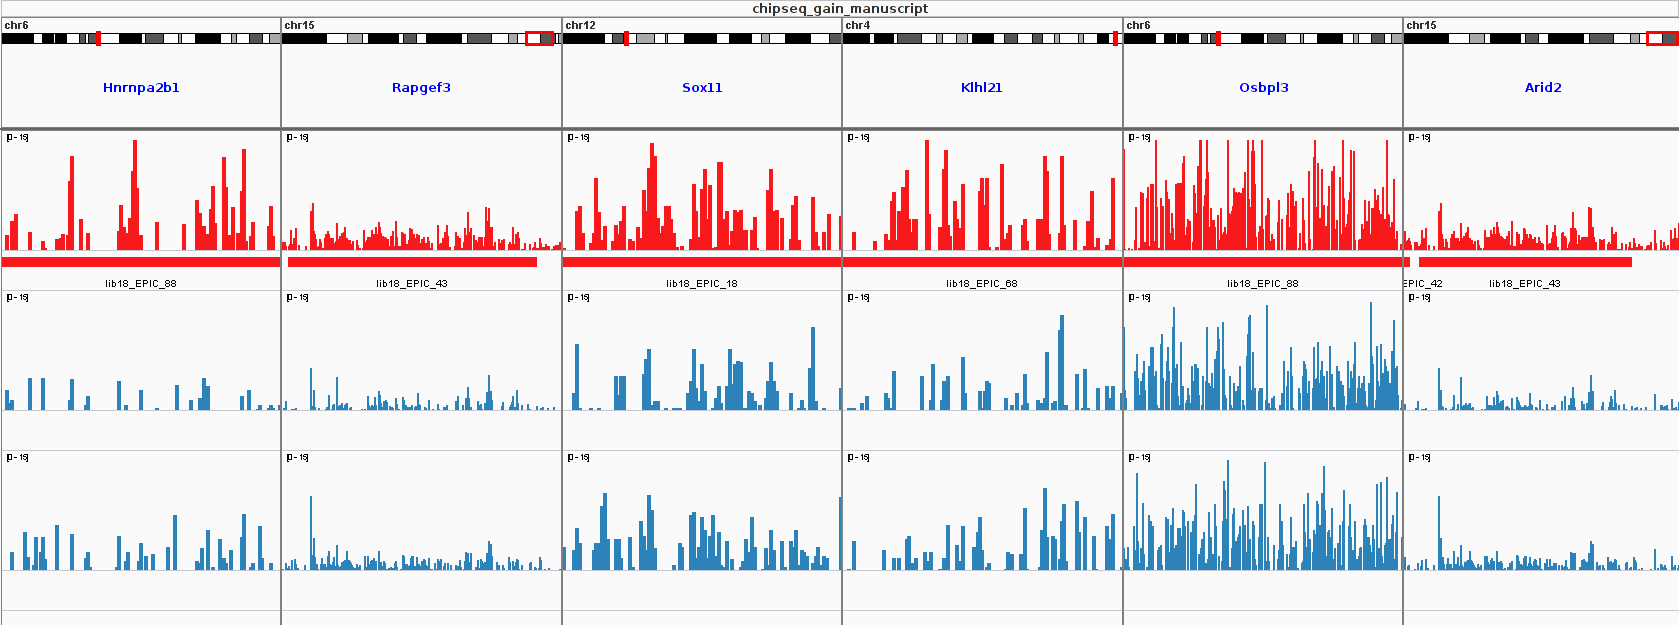
\includegraphics[scale=0.28]{IGV_gain.png}
\scaption{Régions géniques du chromosome 4 identifiées comme marquées dans la condition HD et non marquées dans la condition HDm. Les rectangles sous la librairie HD2 correspondent aux pics détectés par EPIC.
HD2 est représentée en rouge, HDm1 et HDm2 en bleu. La même échelle est utilisée pour chaque librairie : 0 à 15}
\label{gain}
\end{figure}


Pour les régions identifiées comme ayant une "perte de marquage" dans la condition HD par rapport à la condition HDm, les résultats sont beaucoup moins clairs. En effet, nous pouvons observer du signal dans les deux conditions aux mêmes amplitudes mais les pics sont seulement détectés en condition HDm (Figure \ref{perte}). Les pics existent mais avec un FDR très haut. Ainsi, nous ne nous sommes pas concentrés sur l'analyse des gènes spécifiques à la condition HDm pour lesquels nous supposons une sous-estimation du marquage dans la condition HD et/ou une mauvaise attribution du marquage dans la condition HDm.


\begin{figure}[!h]
\centering
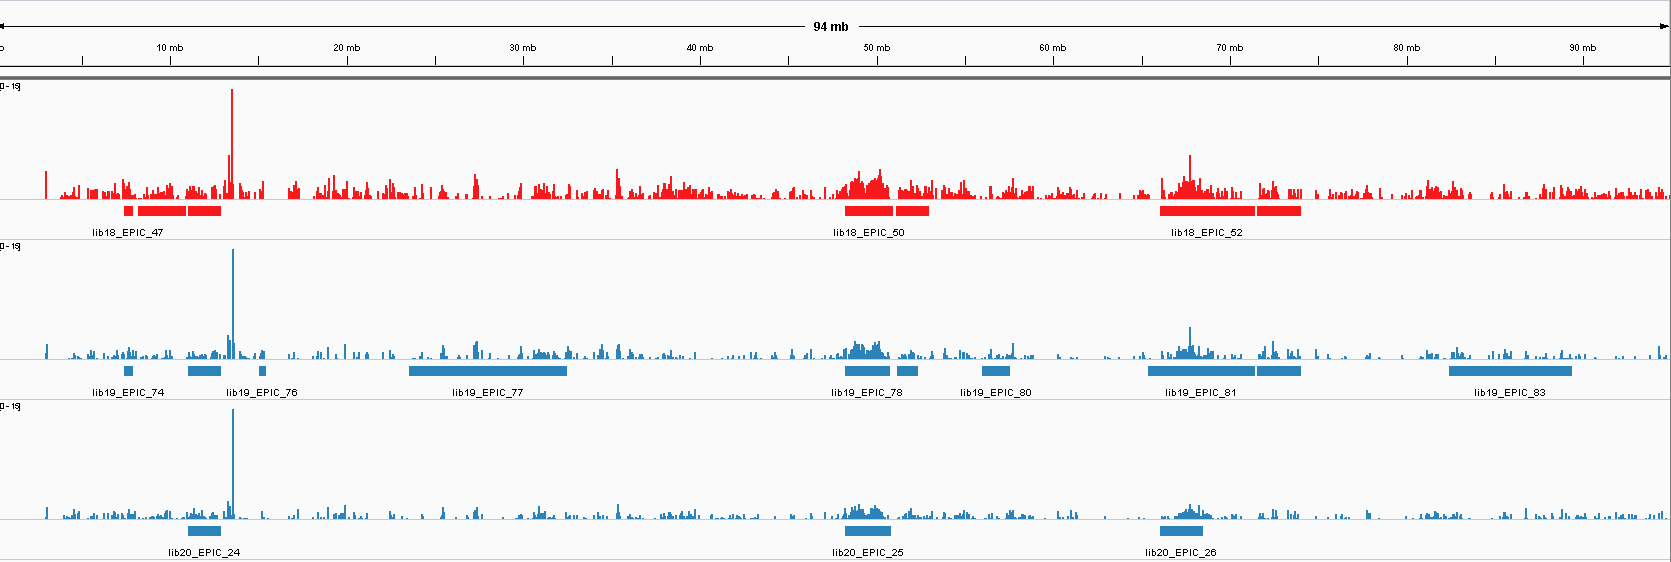
\includegraphics[scale=0.28]{IGV_chr17.png}
\scaption{Régions du chromosome 17 identifiées comme ayant soit pas de modification de la méthylation, soit une perte de la méthylation en condition HD par rapport à la condition HDm.
HD2 est représentée en rouge, et HDm1 et HDm2 en bleu. La même échelle est utilisée pour chaque librairie : 0 à 15}
\label{perte}
\end{figure}


Ainsi l'expression de la TALE-démétylase semble induire une très faible redistribution de la méthylation dans les régions uniques. Les régions identifiées comme ayant une perte de la méthylation dans la condition HD par rapport à la condition HDm sont, visuellement, beaucoup moins convaincantes que les régions ayant un gain de la méthylation.


    \section{Modifications du signal H3K9me3 sur les éléments répétés }
 Le problème de l'analyse globale sur le génome de référence est l'assemblage de mm10 qui contient peu de séquences péricentromériques, pas de télomères, pas de centromères et peu de séquences répétées.
   
   \bigskip
    Pour essayer d'estimer la proportion de reads sur les éléments répétés, la première stratégie a été d'aligner les reads sur une base de données d'éléments répétés (RepBase \cite{repbase}) où la grande majorité des répétitions y sont présentes sous forme de concensus monomériques.
    Les reads ne peuvent pas y être alignés en paired-end, au risque de perdre de l'information pour les répétitions en tandem. 
    En effet, les reads qui chevauchent à la fois un gène et un élément répété, ainsi que les répétitions en tandem, ne pourraient pas être alignés correctement dans RepBase.
    C'est pour cela que seul un mate (R1) du paired-end a été découpé pour atteindre une taille de 35 bp a été aligné (l'alignement du mate R2 contre RepBase a également été réalisé de la même façon pour confirmer les résultats).
 Une fois l'alignement terminé, le nombre de reads sur chacune des répétitions a été compté.
   \newline En parallèle, l'outil RepEnrich2 \cite{pmid25012247} a été utilisé.  Cet outil utilise le génome masqué de repeatMasker pour estimer le nombre de reads sur les répétitions.
   \newline Comme les résultats obtenus avec RepBase et RepEnrich2 sont identiques, seul les résultats obtenus avec RepEnrich2 seront présentés ici.
   
    \bigskip
    En moyenne, pour chaque librairie,  20\% des reads s'alignent sur des éléments répétés. Ce résultat est cohérent avec celui obtenu dans la partie d'analyse des régions uniques où l'on voyait que 20\% des reads filtrés étaient des hits multiples (Table \ref{tab2}).
    \newline
    Pour interpréter  les données générées par RepEnrich2, une ACP globale entre nos librairies a été réalisée (Figure \ref{ACP}).  
    Les dimensions 1 et 2  expliquent le mieux la variabilité.
    La première dimension semble indiquer que la librairie HD2 se comporte différemment des 3 autres librairies (correspond à environ 70\% de la variabilité). Autrement dit, le réplicat HD1 est plus proche des réplicats contrôles que de HD2, son réplicat biologique.
  Ce résultat est identique à celui observé pour les éléments uniques, ce qui confirme le comportement différents de nos réplicats HD.
   Par conséquent, le réplicat HD1 a été écarté pour la suite des analyses.
  
  
   
\begin{figure}[!h]
\centering
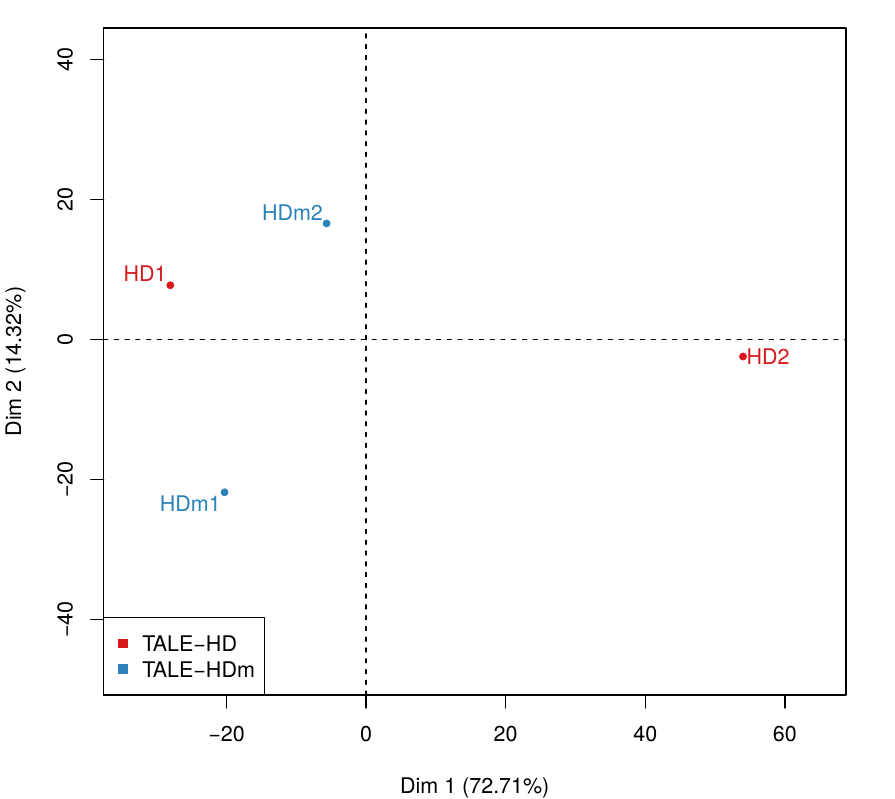
\includegraphics [scale=0.45]{RepBase_PCA.png}
%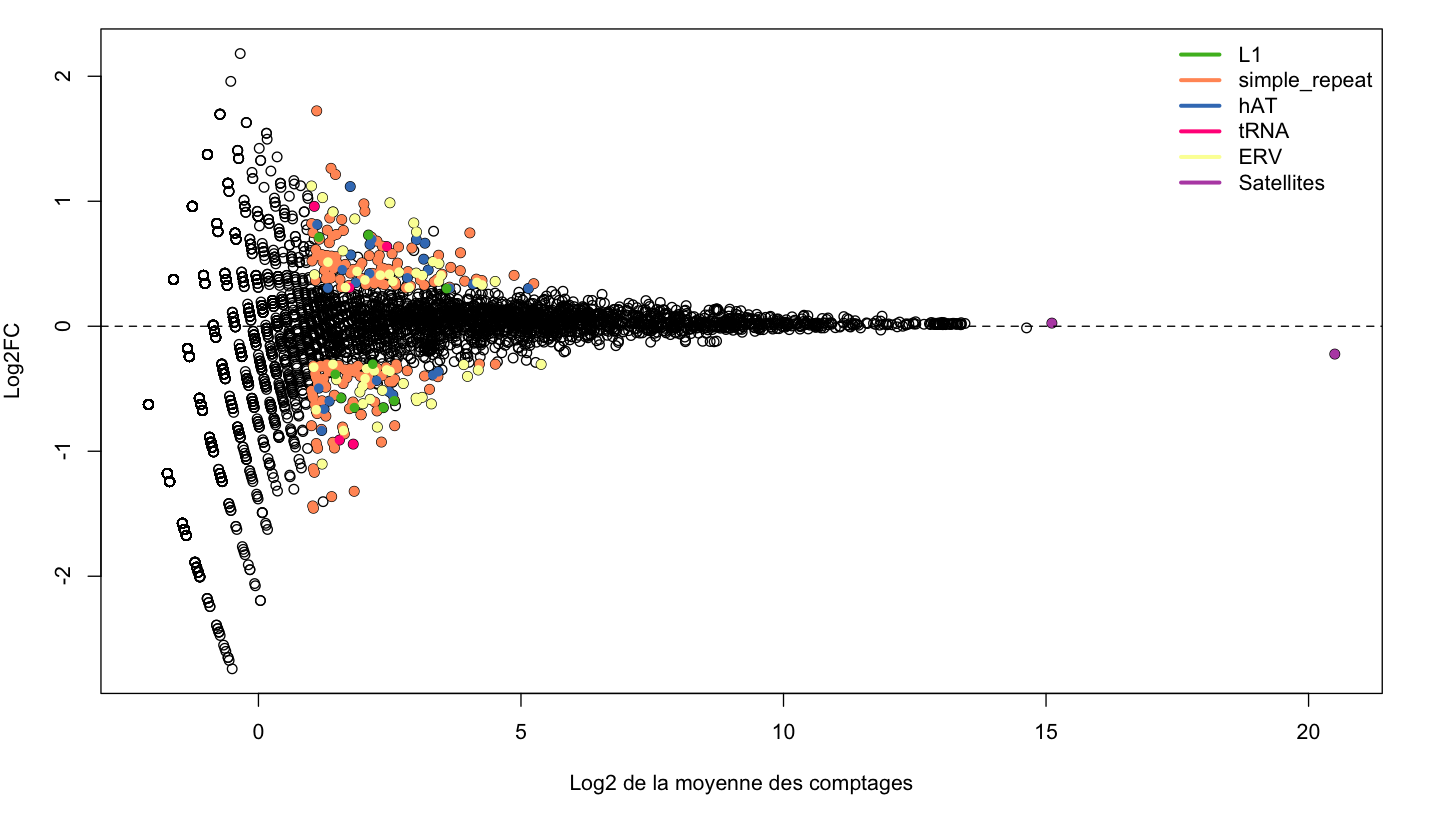
\includegraphics [scale=0.33]{RepEnrich_PCA.png}B
\scaption{ ACP réalisée à partir des comptages de RepEnrich2. Les librairies traitées sont représentées en rouge et les libraries contrôles en bleu.}
\label{ACP}
\end{figure}


Nous cherchons à déterminer les répétitions qui sont significativement enrichies ou appauvries dans la condition traitée par rapport à la condition contrôle. Pour cela, pour chacune des librairies (HD2, HDm1 et HDm2), le nombre de reads s'alignant dans chaque élément répété est déterminé, puis normalisé par le nombre de reads alignés dans la librairie correspondante. Une moyenne, pour chaque élément répété, est calculée pour les librairies contrôles. Cette moyenne sera comparée aux nombres de reads comptés dans la condition traitée (HD2).
Le réplicat HD1 ne faisant plus partie de notre analyse, nous ne pouvons faire une analyse différentielle avec edgeR ou DESeq2.
Nous nous sommes donc limité à l'analyse des Log2FC du nombre de reads par éléments répétés. Pour le calcul des Log2FC, le rapport HD/HDm du nombre de reads normalisés par la taille des librairies pour chaque éléments répétés a été réalisé. Ainsi, un Log2FC négatif signifie qu'il y a plus de signal en HDm qu'en HD, ce qui se traduit par une perte de la méthylation de H3K9me3 en condition traitée. Un Log2FC positif signifie qu'il y a plus de marquage  dans la condition TALE-HD que dans la condition TALE-HDm, ce qui se traduit par un gain de la méthylation en condition TALE-HD.


\bigskip Un MAplot permet de représenter ces Log2FC en fonction du Log2 de la moyenne des comptages (voir matériel et méthodes pour le calcul de cette moyenne) (Figure \ref{Maplot}). Dans ce graphique, chaque point correspond à un élément répété. Plus un point sera à droite du graphique, plus le nombre de reads présents sur la répétition sera important et inversement. Plus un point sera en haut du graphique, plus la répétition sera sur-représentée dans la condition HD par rapport à la condition contrôle et inversement.
    Nous nous intéressons donc aux répétitions qui s'écartent le plus du nuage de points. 
     \newline Les points qui nous intéressent ici sont ceux qui ont un Log2FC supérieur à 0.3 ou inférieur à -0.3 et dont le Log2 de la moyenne des comptages est supérieure à 1.
     Ces points ont été colorés en fonction du type de répétitions.
   
 Les satellites majeurs (point le plus à droite) et mineurs (le deuxième point le plus à droite) sont les répétitions qui ont le plus de comptages.  Le log2FC du satellite majeur, - 0.22, traduit bien une perte de méthylation.
 Il y a donc en moyenne 12\% de zones méthylées en moins dans les satellites majeurs dans la condition HD par rapport à la condition HDm. Ce résultat est cohérent celui décrit précédemment (partie 3. des résultats) qui dénombrait aussi une baisse de 12\% du nombre de reads dans la grande région de satellites majeurs du chromosome 9.
 Le Log2FC du satellite mineur est autour de 0 : il n'y a donc pas de modification de la méthylation dans les centromères.
 Pour les autres types de répétitions (simple\_repeat, ERV, LINE L2, tRNA), le signal est plus compliqué. Il semble en effet que selon le sous-type d'élément considéré, nous observons soit une perte, soit un gain de méthylation.


\bigskip
Ainsi, on observe une petite redistribution de la marque dans certains éléments répétés. Toutefois, aucune famille d'éléments répétés ne semble préférentiellement enrichie.
Il semble que de nombreux éléments répétés présentent aussi une perte de méthylation dans la condition TALE-déméthylase par rapport à la TALE-déméthylase inactive.


     
\begin{figure}[!h]
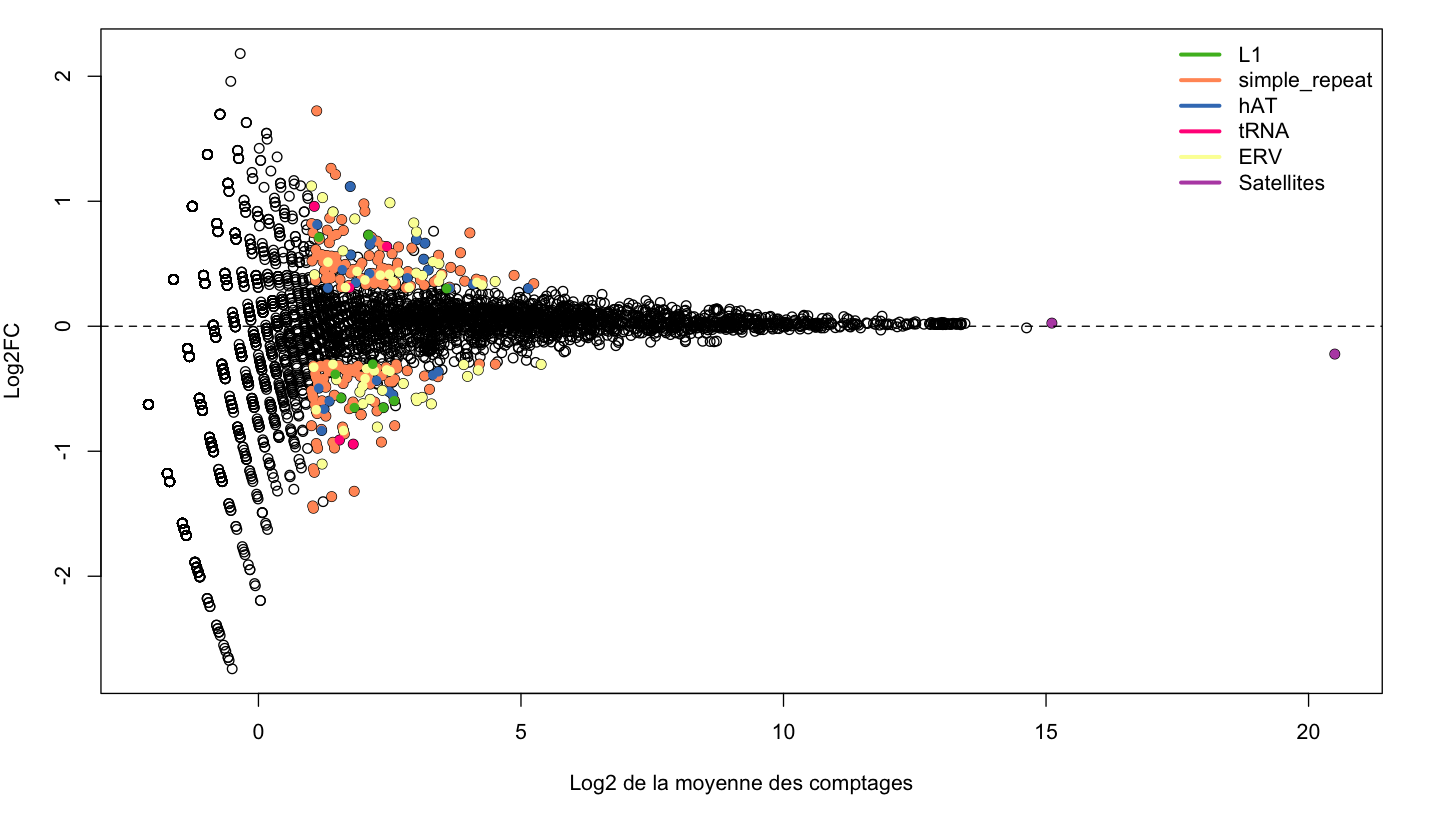
\includegraphics [scale=0.35]{RepEnrich_PCA.png}
%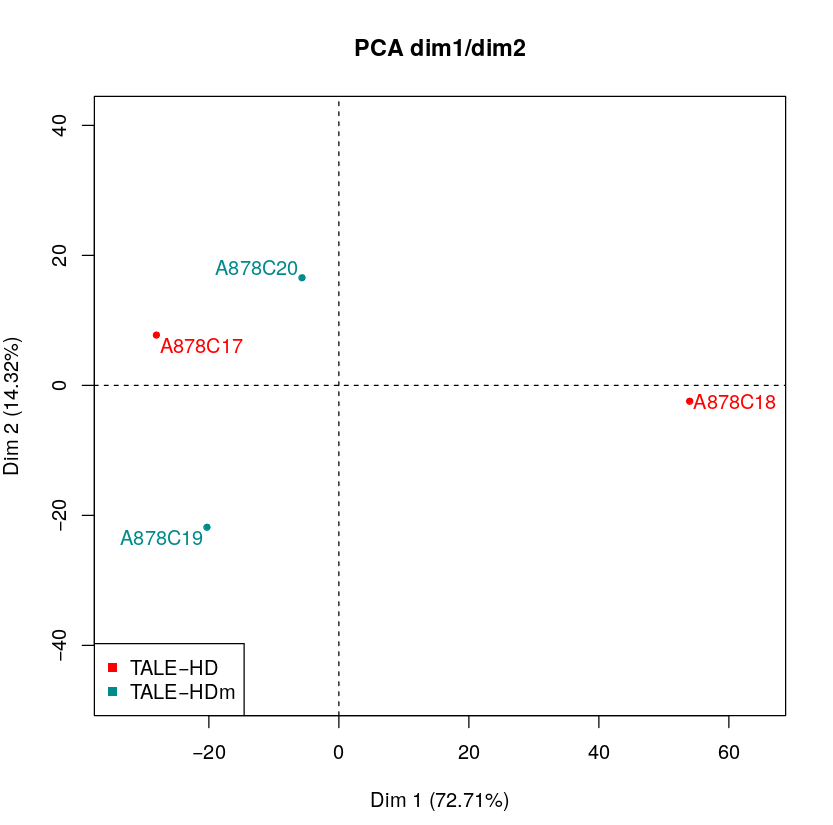
\includegraphics [scale=0.45]{RepBAse.png}B
\scaption{MAplot  pour les comptages de RepEnrich2: pour chaque échantillon, les comptages ont été normalisés par la taille de leur librairie. Ensuite, les comptages sur les répétitions entre les deux réplicats contrôles sont mis en communs. Enfin, le log2FC du rapport traité sur contrôle est calculé ainsi que la moyenne des comptages HD2 et HDm.}
\label{Maplot}
\end{figure}


\newpage
\chapter*{{
\vspace*{-2cm}}Discussion et perspectives}
\setcounter{section}{0}
\addcontentsline{toc}{chapter}{Discussion}


 
 \section {Comportement des réplicats}

Lors de l'analyse des régions uniques et des régions répétées, nous nous sommes rendu compte qu'une des deux librairies traitées (HD1) se comportait comme les librairies contrôles  et nous avions fait le choix de l'écarter du jeu de données. En effet, comme les images de microscopie suggéraient une redistribution du marquage H3K9me3 dans les cellules exprimant la TALE-HD, nous avons supposé que la librairie HD2,  
présentant une répartition de H3K9me3 bien différente des librairies contrôles (visibles grâce aux ACP), était celle qu'il fallait conserver.
\newline
Le fait que  la librairie HD1 présente un signal proche de celui observé dans les librairies contrôles pourrait venir de la variation du taux d'expression de la TALE-HD dans ces cellules.
En effet, pour permettre l'expression de la TALE-HD ou de la TALE-HDm dans les cellules, celles-ci doivent être transfectées avec les plasmides correspondant. Cette transfection permet de faire "rentrer" dans les cellules un nombre variable de copies de plasmides. L'équipe a pu montrer qu'il y avait une forte corrélation entre le niveau d'expression de la TALE-HD et la perte de H3K9me3 dans les régions péricentromériques (plus la TALE est exprimée, moins il y a de signal H3K9me3). Ainsi, il est possible que les cellules de la condition HD1 aient, en moyenne, un plus petit nombre de plasmides exprimant la TALE-HD que les cellules de la condition HD2. 
\newline
Cependant cette hypothèse ne semble pas se vérifier au vu des résultats du ChIP-Seq au niveau des satellites majeurs du chromosome 9, qui présentent une diminution du signal de 12\% identique dans les librairies HD1 et HD2.  Il y a donc bien une diminution de la méthylation sur un GSAT en cohérence avec l'expérience, malgré un comportement global plus proche d'un contrôle.
 \newline Il est également possible que ce soit la librairie HD1 qui ait correctement fonctionné et que HD2, pour une raison quelconque, se comporte très différemment des autres. Avec seulement deux réplicats, nous ne pouvons pas savoir lequel a le mieux fonctionné.
%La librairie HD1 étant celle qui possède le moins de reads (2x 29 milliions), il est également possible qu'il n'y ai pas assez de profondeur de séquençage pour observer quelque chose.
 \newline Il est aussi possible que les réplicats HD1 et HD2 correspondent à une réalité biologique qui se traduirait par une redistribution de H3K9me3 aléatoire sur le génome, et donc selon les cas, il y aurait plus ou moins de redistribution ou une redistribution variable. 
 
  \bigskip
  En tout état de cause, l'existence actuelle de deux réplicats ne permet pas de trancher.
L'équipe a donc prévu de relancer de nouveaux réplicats pour chaque condition à la rentrée. L'analyse par ACP pourra alors nous renseigner sur la diversité globale du comportement standard d'un réplicat.

 
 \section{Suppression des biais de PCR}
 Pour ne garder que les reads uniques, plusieurs filtres ont été appliqués après l'alignement sur le génome de référence. La suppression des biais de PCR avec l'option "rmdup" ne gère pas bien les reads répétés en paired-end.  En effet, cette option utilise le paired-end comme s'il s'agissait de single-end. 
 Ainsi, si le mate R1 d'un read est localisé au même endroit qu'un autre mate d'un autre read, il sera supprimé même si le mate R2 est localisé de manière unique à une localisation génomique, ce dernier étant conservé. Le fichier de sortie comporte donc des singletons ayant perdu, à tort, un mate. Ces singletons représentant seulement 1 \% de la taille des  librairies, l'analyse les a pour le moment ignoré. Toutefois, l'écriture d'un script pour le traitement des ces reads est à envisager pour la suite du projet.
  
   \section {Normalisation par l'Input}
  Le séquençage de l'Input en ChIP-seq est le standard actuel. Il est utilisé en particulier comme normalisateur de bruit au moment de la détection des pics. Toutefois, son utilisation comme normalisateur local d'éléments comparés 2 à 2 posent débats : il semble assez clair que l'Input sert à vérifier les zones du génome qui pourraient être sur-séquencées, mais que le biais local ne peut à lui seul être géré par l'Input.
 \newline Nous avons testé de nombreuses méthodes de normalisation au cours de ce stage, comme la soustraction de l'Input à l'IP, le ratio de l'IP par l'Input et même le log2 ratio du signal Input au signal IP. 
 Le choix de la méthode de normalisation a posé problème pour le calcul des Log2FC sur les éléments répétés. En effet,  la normalisation de l'Input par soustraction pouvant produire des résultats négatifs, le calcul du Log2FC correspondant devient alors délicat (il n'est pas possible de calculer le Log2FC d'une valeur négative). Pour pallier ce problème, les résultats négatifs avaient tout d'abord été ramenés à zéro, ce qui avait eu pour conséquence de produire des Log2FC égaux à +/-Inf. Cette méthodologie ne nous paraissait pas pertinente car des éléments répétés comme des satellites mineurs, qui normalement ne doivent pas avoir une grande variation de la méthylation, se retrouvaient avec des valeurs de Log2FC très grandes.
  \newline
  Ainsi, il nous est apparu que, dans notre cas d'étude, il était plus pertinent d'utiliser uniquement l'Input comme normalisateur pour la détection de pics afin de déterminer des régions "enrichies" en H3K9me3 par rapport au bruit global sur le génome, mais de ne pas le prendre en compte quand il s'agissait de déterminer un taux d'enrichissement local sur des régions spécifiques du génome .
  \newline
   En faisant ce choix de normalisation pour l'étude des régions répétées et pour estimer le taux de perte de la méthylation  sur les satellites majeurs, il est possible que l'on sous-estime les taux d'enrichissement  ainsi que les taux de perte de la méthylation dans la condition HD par rapport à la condition HDm. 
  
  
  \bigskip
  Toutefois, il semblerait que l'utilisation de l'Input spécifique à l'IP séquencé puisse être une solution. En effet, pour \cite{norma}, la normalisation par le nombre total de lectures alignées a pour effet de ramener le niveau de l'expérience traitée au même niveau que l'expérience contrôle dans la mesure où le signal est quantifié comme un simple pourcentage de lectures alignées. Ainsi, une diminution de 50\% du signal entre les deux conditions ne peut pas être déterminée avec cette méthode de normalisation.  
  Orlando et ses collaborateurs proposent une méthode alternative : la méthode Spike-in(SI). Cette technique consiste à mettre une proportion fixe de chromatine d'une espèce exogène de référence dans chaque tube avant le séquençage. Ainsi, le nombre de lectures alignées sur le génome exogène permettrait  d'effectuer la normalisation de chaque échantillon (IP et Input) car la chromatine exogène sera dans le même état dans toutes les conditions. Enfin, l'Input est soustrait à chaque IP et les valeurs négatives qui pourraient en résulter sont ramenées à zéro.  
\newline Actuellement, nous ne disposons que d'un seul Input (qui est celui de HD2) et nous ne pouvons donc pas appliquer cette méthodologie.  Toutefois, cette option est envisageable pour les nouveaux séquençages à venir.
 \section{Choix des paramètres et des algorithmes pour la détection de pics}
 Pour effectuer l'analyse sur les régions uniques nous avons testé deux détecteurs de pics : MACS2 \cite{MACS} et EPIC \cite{SICER}.
 Ces deux détecteurs sont tous les deux décrits comme étant adaptés à la détection de marques hétérochromatiniennes diffuses comme H3K9me3.
\newline
 MACS2 a dans un premier temps été utilisé avec les paramètres par défaut (Annexe - Figure \ref{MACS2D}).  Nous nous sommes rendu compte que sur de nombreuses régions, des pics n'étaient pas détectés et inversement,  que les pics détectés n'étaient pas forcément bien placés par rapport au signal observé.  De très nombreux paramètres de MACS2 ont été testés comme la taille de fenêtres (Annexe - Figure \ref{MACS2T} et Table 5), les "qvalues", et "nomodel" (pas d'utilisation de modèle statistique) sans grand changement sur la détection des pics. Une recherche dans les pages GitHub de MACS2 a confirmé ce problème : MACS2 serait défectueux dans sa recherche de pics larges et devrait être réimplémenté (datant du 14 mai 2018).

\bigskip
Le second algorithme reconnu pour détecter des marques chromatiniennes larges est SICER \cite{SICER}. Or, SICER ne gère pas les données paired-end.  C'est pour cette raison que nous avons décidé d'utiliser EPIC  \cite{SICER} qui est une réimplémentation de SICER pour gérer le paired-end. Pour EPIC, la taille des fenêtres a été fixée à 20 kb et les pics ayant un FDR inférieur à 1e-20 ont été conservés.
\newline
Le choix de ces deux paramètres peut être considéré comme stringent puisque que sur de nombreuses régions du génome, des pics ne sont pas présents dans la librairie HD2 alors que du signal est observé (Figure \ref{circoss}). Ces pics existent (Annexe - Figure \ref{circosTout}), mais ont un FDR très mauvais (supérieur à 1 e-3).  Il semblerait donc qu'avec EPIC, les pics des réplicats de la condition HDm sont détectés avec un bon FDR alors que les pics de la condition HD sont détectés avec un mauvais FDR.
 \newline
Il est possible que la mauvaise détection de pics pour la librairie HD2 soit corrélée au signal global plus haut de cette librairie par rapport au signal des librairies HDm.
Pour que les pics soient en adéquation avec le signal global observé, une solution serait de fixer des seuils différents de FDR dans les conditions HD et HDm, ce qui demanderait de valider en amont le choix de ces deux seuils différents.
\newline Une autre solution serait de tester de nouveaux détecteurs de pics n'utilisant pas la même stratégie.
En effet, il est possible que l'analyse en fenêtres glissantes effectuée par ces détecteurs de pics ne soit pas adaptée pour nos librairies : si la librairie HD2 présente une hyper-méthylation globale du génome, les détecteurs peuvent ne pas être adaptés. 

\bigskip
Le choix de ces différents algorithmes et des différents paramètres qui leurs sont associés a très fortement impacté les analyses. En effet,  en choisissant EPIC comme détecteur de pics avec une taille de fenêtres à 20 kb  et en fixant le seuil du FDR à 1e-20, la redistribution du signal n'est que peu visible dans les régions uniques et nous y observons même une forte baisse du nombre de nucléotides couverts par la marque H3K9me3. Ainsi, 260 gènes gagnent du marquage H3K9me3 quand environ 3600 en perdent potentiellement. En d'autres termes, cela signifierait qu'environ 3600 gènes seraient déméthylés, donc réactivés, ce qui remet en cause la survie de la cellule.
De plus, nous avions remarqué que les régions qui gagnaient du marquage H3K9me3 en condition TALE-HD étaient cohérentes avec le signal visualisé sur IGV, ce qui n'était pas le cas pour la perte de marquage : il semblerait donc que, parmi ces 3600 gènes, beaucoup ne subissent en réalité aucune modification de la méthylation ; , ce chiffre est donc probablement très sur-estimé.


   \section {Gènes marqués dans les deux conditions}
   Lors de l'analyse des régions uniques, nous avions montré que certains gènes étaient identifiés à la fois en HD et en HDm. 
   Pour qu'un gène soit marqué dans les deux conditions, il peut être soit marqué à des positions différentes en HD et HDm, soit marqué aux mêmes positions en HD et en HDm (Table 3 de la partie Résultats). Dans ce dernier cas, il est possible qu'il y ait une modification de l'intensité du signal. Ces conditions n'ont pas été explorées au cours du stage, par manque de temps. Toutefois, la modification de l'intensité du signal pourrait être analysée en réalisant un comptage du nombre de lectures sur les différents pics avec htseq-count \cite{Htseqcount} par exemple.


  \section{Eléments répétés}
L'analyse de la redistribution sur les éléments répétés représente un véritable challenge dans la mesure où les séquences répétées ne sont pas ou peu assemblées dans le génome de référence et où peu de méthodes existent à l'heure actuelle pour estimer la proportion de reads sur ces éléments répétés. Nous avons utilisé deux méthodes différentes (RepBase et RepEnrich),  donnant chacune des résultats équivalents, renforçant ainsi les hypothèses que nous avons formulées concernant la redistribution de la marque H3K9me3 sur les éléments répétés.
\newline Nous avions remarqué que la marque H3K9me3 était redistribuée sur certains éléments répétés mais aucune famille préférentiellement choisie n'avait pu être déterminée. 
Il est donc possible que la redistribution soit stochastique d'une cellule à une autre 
ou que l'intensité du signal diffère d'une cellule à une autre, que ce soit en lien ou non avec la quantité de plasmides transfectés et de la TALE exprimée.
\newline
Parmi les éléments répétés enrichis dans la condition TALE-HD, certains LINE sont identifiés. Ces séquences étant très abondantes dans le génome de la souris, il est probable que la redistribution de la marque H3K9me3 se fasse sur des LINE de façon aléatoire, le tout est de déterminer si cet enrichissement des LINE est statistiquement probant.. Nous pouvons également noter que les LINE correspondent à de l'hétérochromatine facultative. Ce sont donc des séquences d'ADN répétées qui peuvent être plus aptes à subir des modifications, que ce soit de la méthylation ou de la déméthylation en H3K9me3. Une analyse statistique pour déterminer si la redistribution sur les LINE est significative sera réalisée une fois les nouvelles librairies séquencées. 
\newline
Le fait que le centromère présente de la méthylation en H3K9 peut être surprenant. En effet, la présence de la marque H3K9me3 au centromère fait débat dans la communauté scientifique. Le consensus actuel fait plutôt état d'une absence de H3K9me3 au centromère au profit de H3K9me2.
Toutefois, quelques études \cite{Discu1}, \cite{Discu2} montrent que H3K9me3 pourrait se diffuser du péricentromère au centromère. 
Il n'est donc pas surprenant de trouver du signal dans notre étude, d'autant plus que l'utilisation d'anticorps pour l'expérience de ChIP-Seq permettent  par la fixation au péricentromère de récupérer des séquences centromériques adjacentes.

 \chapter*{{
\vspace*{-2cm}}Conclusion}

En conclusion, j'ai développé une méthode d'analyse de la marque H3K9me3 permettant d'étudier séparément les régions uniques et répétées du génome. Ce projet s'intègre dans l'analyse plus globale du rôle de H3K9me3 au péricentromère.

\bigskip
Tous les paramètres du protocole ne sont pas encore tous opérationnels, en particulier le filtre des biais de PCR et les paramètres de la détection de pics.
\newline
Les expériences de microscopie en laboratoire montrent qu'en déméthylant les satellites majeurs des péricentromères des chromosomes de souris, une redistribution de la marque semble s'opérer sur le reste du génome sur certains chromosomes métaphasiques étalés.
Cette redistribution semble être confirmée par les analyses de ChIP-Seq si on considère l'augmentation global du signal sur HD2.  Toutefois, cette redistribution ne peut être statistiquement confirmée dans la mesure où nous avons travaillé, pour le moment, avec un seul réplicat TALE-déméthylase. 

\bigskip 
Un nouveau séquençage de deux librairies plus profondes est prévu pour tenter de voir si le signal de la librairie HD est complètement stochastique d'une librairie à une autre (ACP éclatée) ou si, au contraire, il est possible d'approcher une redistribution ciblée.
\addcontentsline{toc}{chapter}{Conclusion}
\newpage


\newpage
\chapter*{{\vspace*{-2cm}}Glossaire}


\begin{description} 

\item [ACP : ]  Analyse en composante principale
\item [FDR : ]  False Discovery Rate
\item [GFP :  ] Green Fluorescent Protein
\item [GSAT :  ] Satellites majeurs des chromosomes de souris
\item [HA :  ] hémagglutinine
\item [HD (1 et 2) : ] les deux réplicats traités à la TALE-HD-GFP
\item [HDm (1 et 2) : ]  les deux réplicats contrôles traités à la TALE-HDmutée-GFP
\item [H3K9me3 : ]  Triméthylation de la lysine 9 sur l'Histone H3
\item [Mapping : ] Etape d'alignement des reads sur un génome de référence
\item [Mate :  ] dans le cadre d'un séquençage paired-end, une des extrémités du read
\item [Read : ]  séquence obtenue en sortie de séquenceur pour un fragment d'ADN
\item [RPKM : ] Reads Per Kilobase Million. Dans notre cas, le RPKM correspond aux librairies divisées par leurs tailles
\item [TALE :  ] transcription activator-like factor

\end{description}

\newpage
\chapter*{{
\vspace*{-2cm}}Bilan personnel}
\setcounter{section}{0}
Ce stage de cinq mois et demi a été très enrichissant pour moi car il m’aura permis d’avoir une première expérience dans le milieu de la recherche en bioinformatique.
J’ai pu approfondir mes connaissances sur le traitement des données issues de séquençage et développer mes compétences personnelles. En effet, j'ai pu améliorer ma communication au sein d'une équipe en apprenant à synthétiser mes avancées pour les présenter à la fois à  des bioinformaticiens et  à des biologistes. J'ai également pu développer mon autonomie et la confiance en soi dans la mesure où j’ai était amené à prendre des responsabilités.

\bigskip
Mes activités au cours du stage m’ont permis de mettre en oeuvre les compétences acquises au cours des deux années de master, en particuliers, en python lors de la mise en commun des pics entre les réplicats, en R pour la réalisation des graphiques et en bash lors de l'automatisation de certaines étapes du protocole. J’ai  pu développer mes aptitudes en matière de représentation graphique en apprenant à manipuler les circos.
\newline
Mes connaissances en biologies ont été fondamentales pour, d’une part comprendre le contexte du stage, et d’autre part, produire une analyse adaptée à la problématique posée.

\bigskip
Forte de cette expérience, j’aimerai beaucoup par la suite essayer de m’orienter vers l'analyse de données NGS. 
\bibliographystyle{apalike} 
\bibliography{biblio}  

\begin{appendices}

\newpage
\section{Nombre de reads s'alignant sur les satellites majeurs assemblés dans le génome de référence mm10}

\begin{table}[!htb]
\centering
 \begin{tabular}{|p{1.5cm}|p{2cm}|p{2cm}|p{1.5cm}|p{2cm}|p{2cm}|}

\hline
  & Librairie TALE-HD rep1 & Librairie TALE-HD rep2 & Librairie TALE-HD-mutée rep1&  Librairie TALE-HD-mutée rep2 &  input \\
\hline
chrs 14 & 974065 & 1750736 &  1260841 & 1397532 & 1346662    \\
\hline
chrs 2 & 232199 &  4183913 & 3048944& 3295233 & 4105551   \\
\hline
chrs 9 & 1230711 & 2256586 & 1652105 & 1793294 & 2167302  \\
\hline
Total & 4788209& 8476719 & 6177731 & 6704145 & 8226794 \\
\hline
\end{tabular}
\scaption{Nombre brut de lectures s'alignant sur les satellites majeurs présents dans l'assemblage du génome mm10. Ici,  seuls les comptages pour les chromosomes ayant le plus de reads ainsi que le nombre total de reads s'alignant sur tous les satellites majeurs sont reportés. }
\label{tab3}
\end{table}


\newpage
\section{Détection de pics avec MACS2}
\subsection{Paramètres par défaut}
\begin{figure}[!h]
\centering
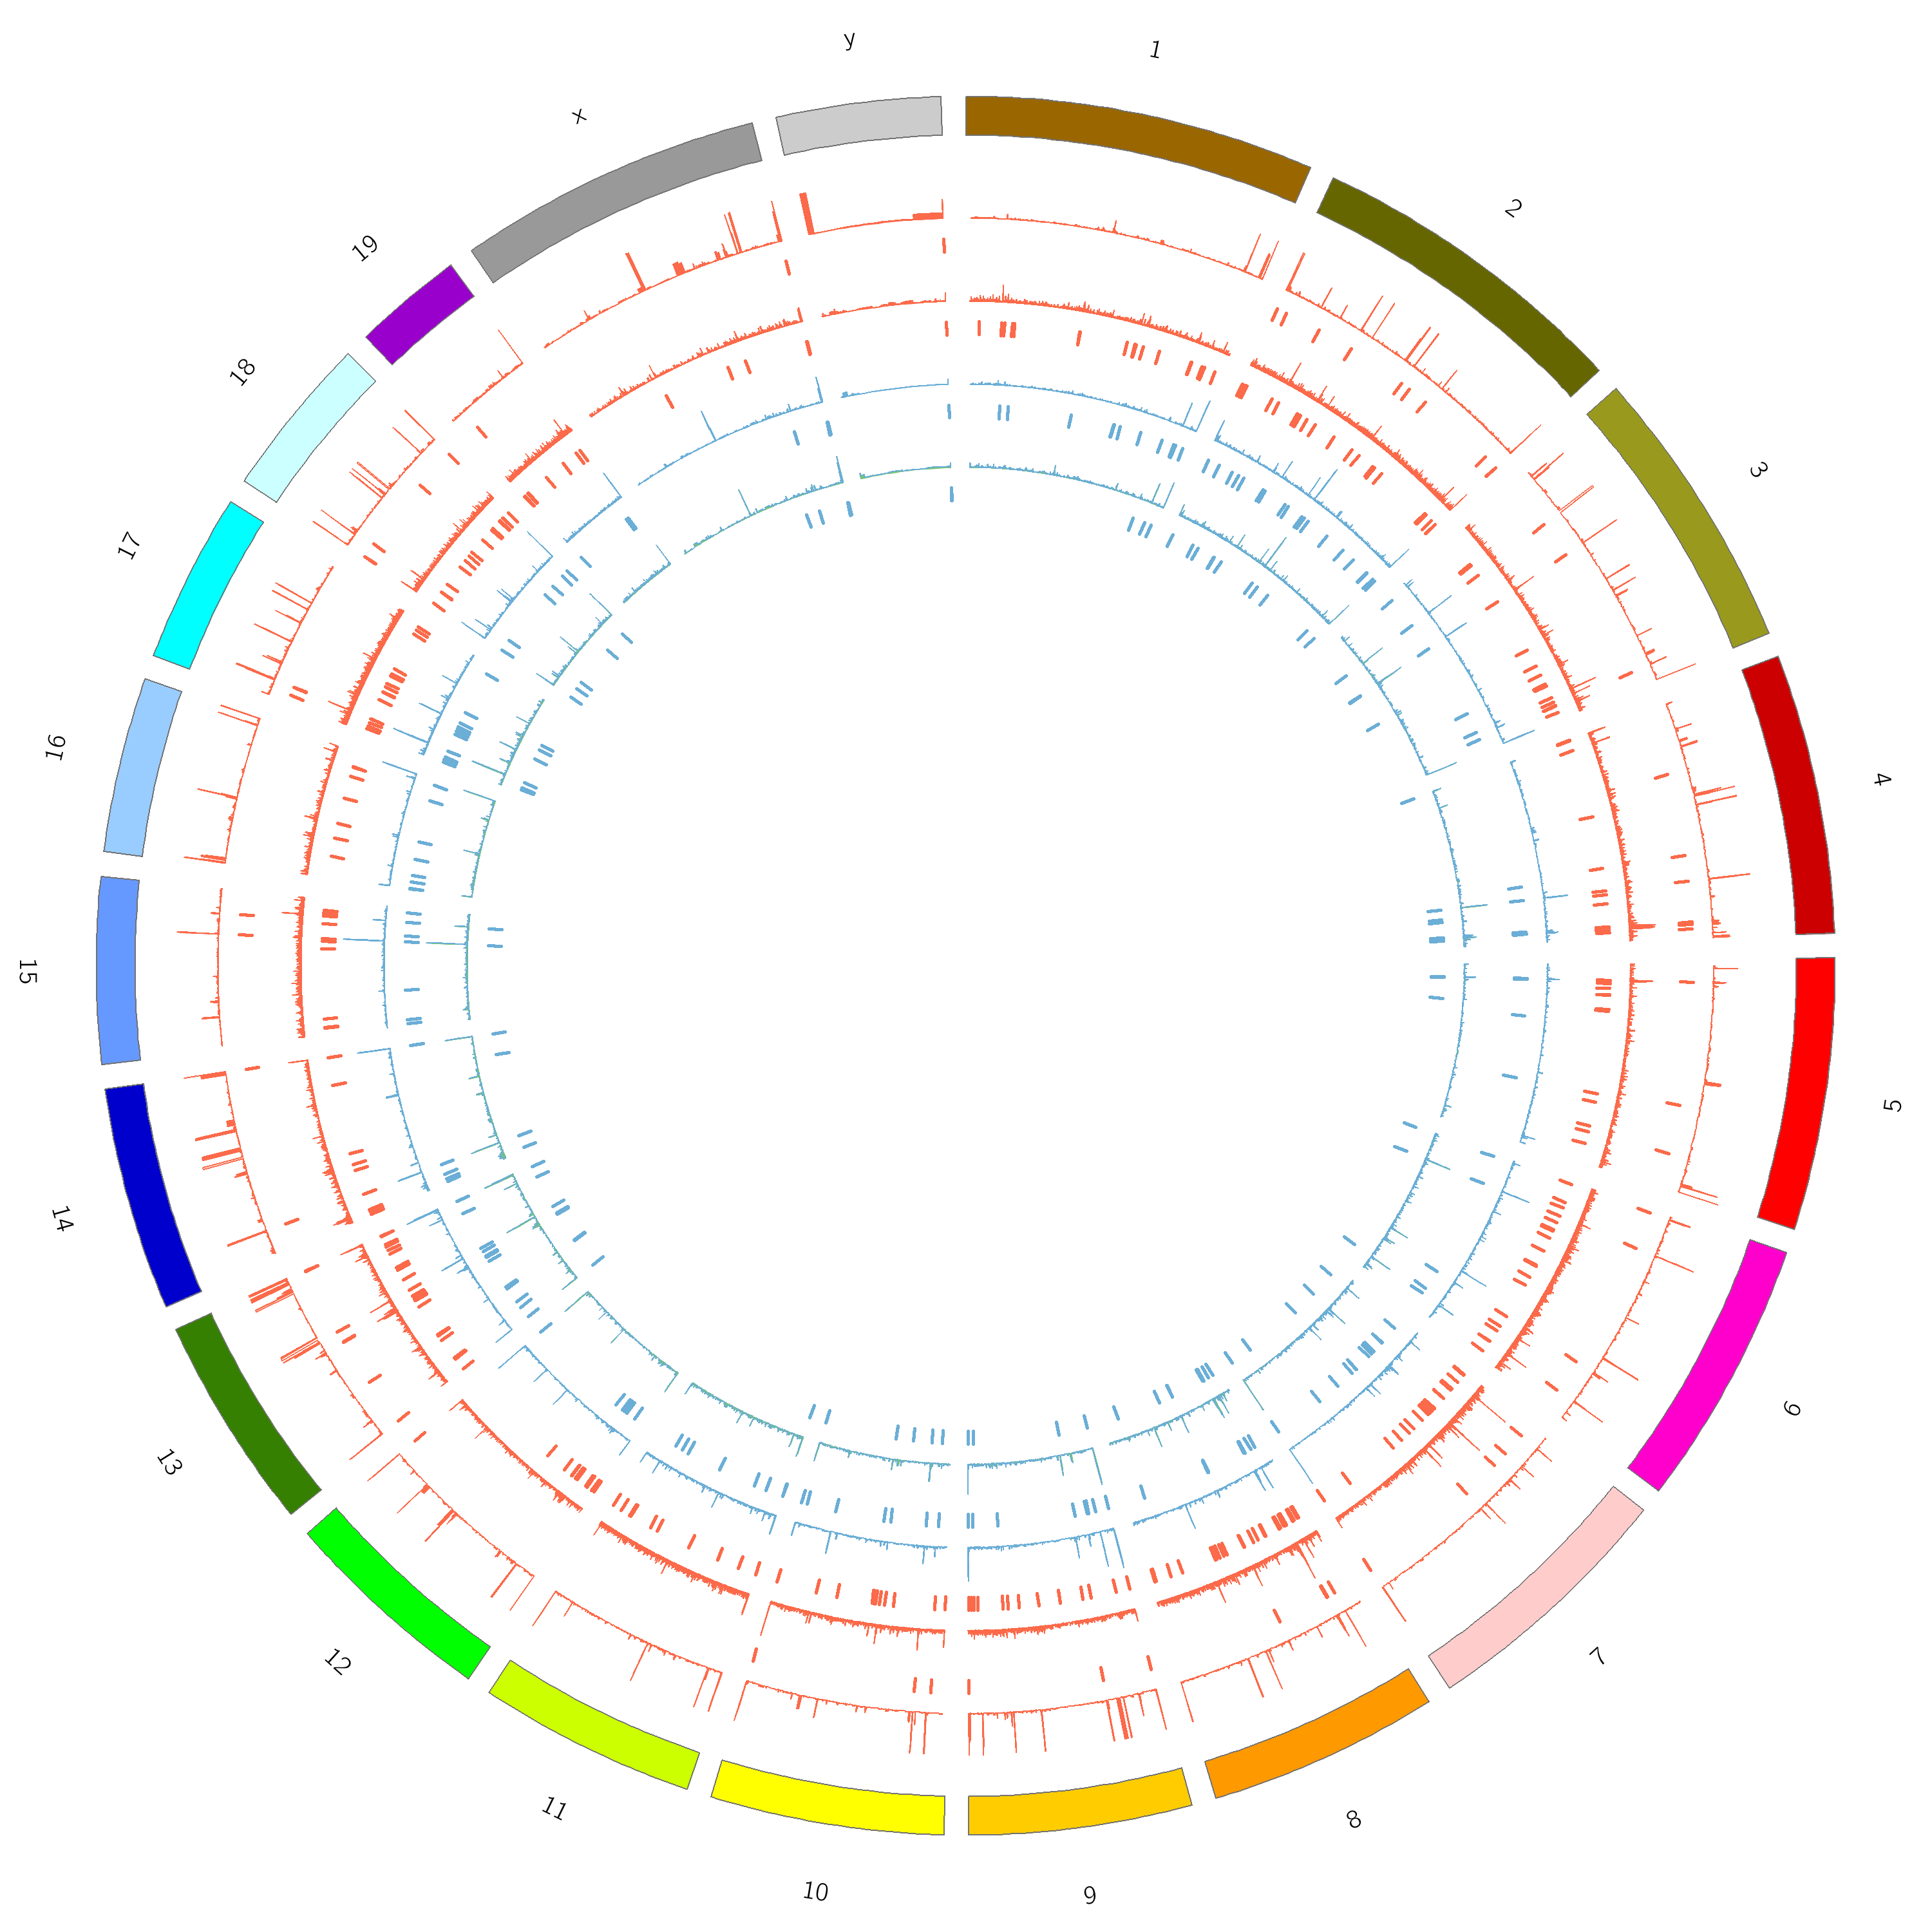
\includegraphics [scale=0.2]{circosMacs.png}
\scaption{Répartition du signal normalisé Ip-Input pour les différentes librairies (après filtre de la redondance).  Les librairies traitées sont en rouges et les librairies contrôles en bleues.
Les pics obtenus avec MACS2 paramètres par défauts sont représentés par des rectangles sous chaque signal leur correspondant.
}
\label{MACS2D}
\end{figure}

\newpage
\subsection{Test de différents paramètres de MACS2}
\begin{figure}[h]
\centering
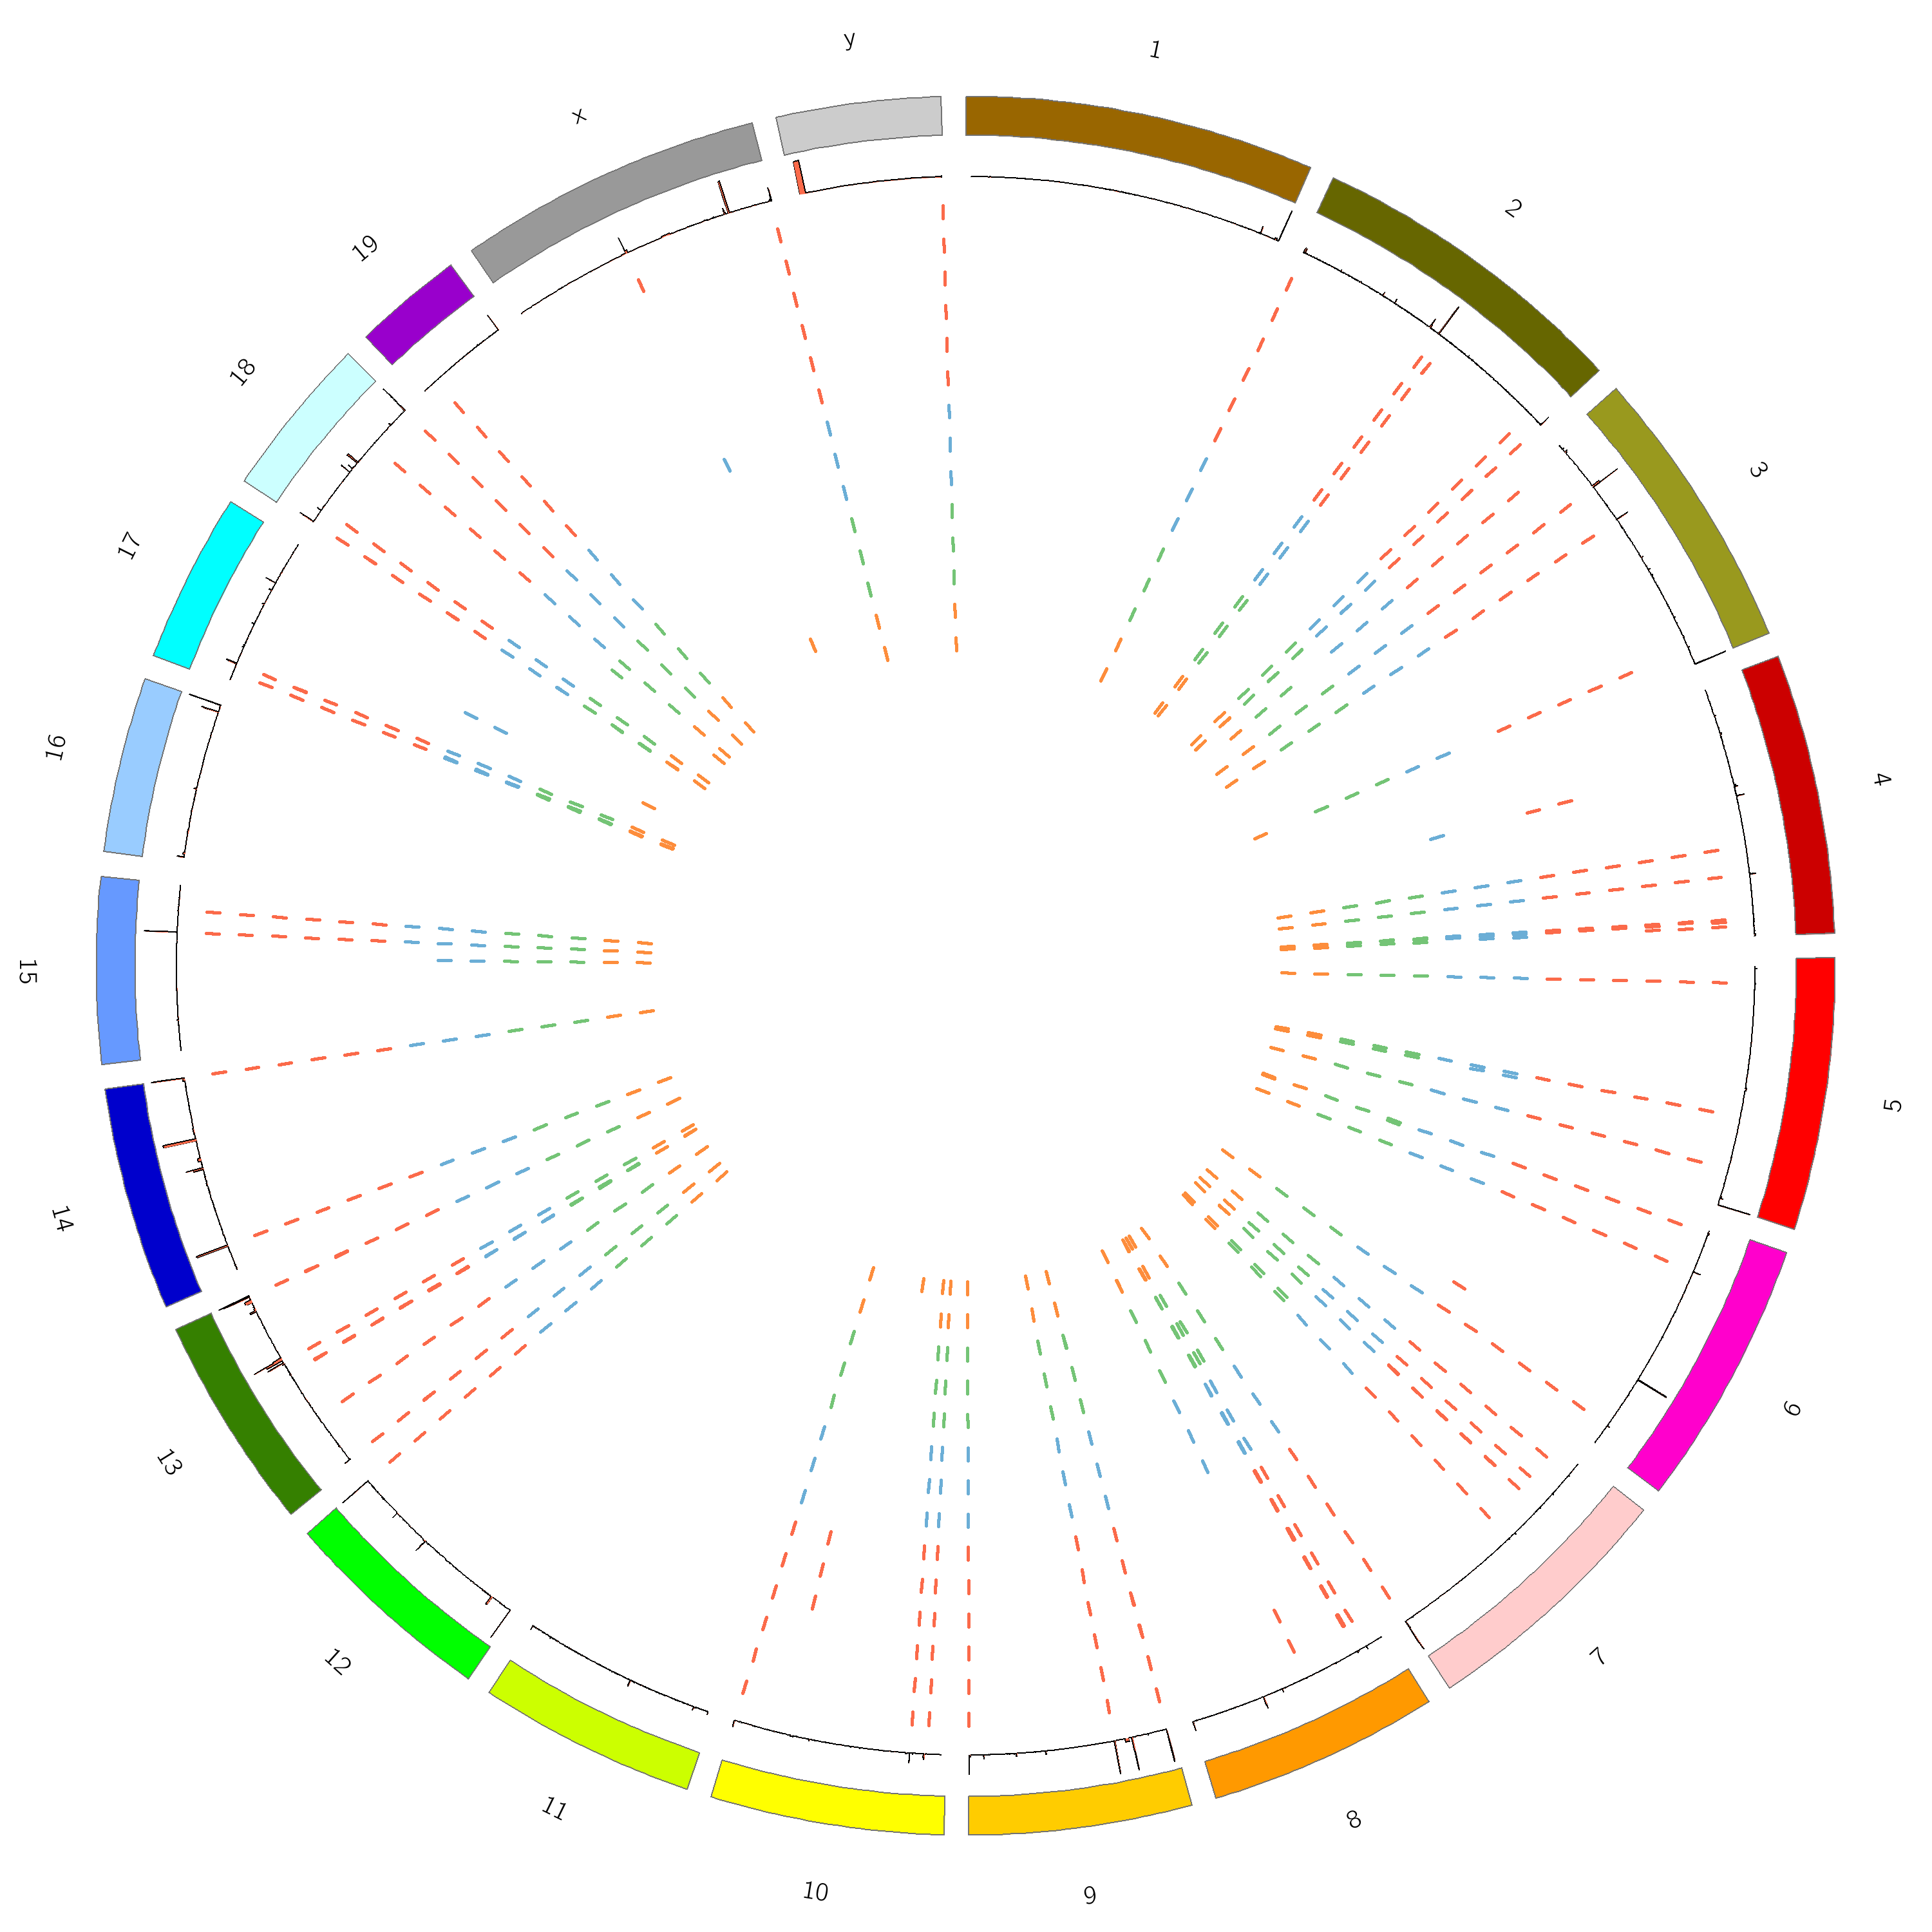
\includegraphics [scale=0.16]{circos_signal_peak_17_diffPeaks.png}
\scaption{Illustration des pics détectés par MACS2 sur la librairie HD1 quand on fait varier différents paramètres. Les paramètres testés - de l'extérieur vers l'intérieur - sont présentés dans la Table 5. }
\label{MACS2T}
\end{figure}

\begin{table}[!htb]
\centering
 \begin{tabular}{|p{0.333\linewidth}|p{0.333\linewidth}|}
\hline
  slocal &  llocal \\
\hline
500 & 1000    \\
550 & 1050    \\
600 & 1100    \\
650 & 1150    \\
700 & 1200    \\
750 & 1250    \\
\hline
500 & 5000    \\
600 & 6000    \\
700 & 7000    \\
\hline
300 & 10 000    \\
350 & 10500    \\
400 & 11000    \\
\hline
500 & 100 000    \\
300 & 100 000    \\
\hline
\end{tabular}
\scaption{Les différents paramètres qui ont été testés pour MACS2}
\end{table}


\clearpage
\section{Pics EPIC non filtrés}
  \begin{figure}[!h]
    \centering
    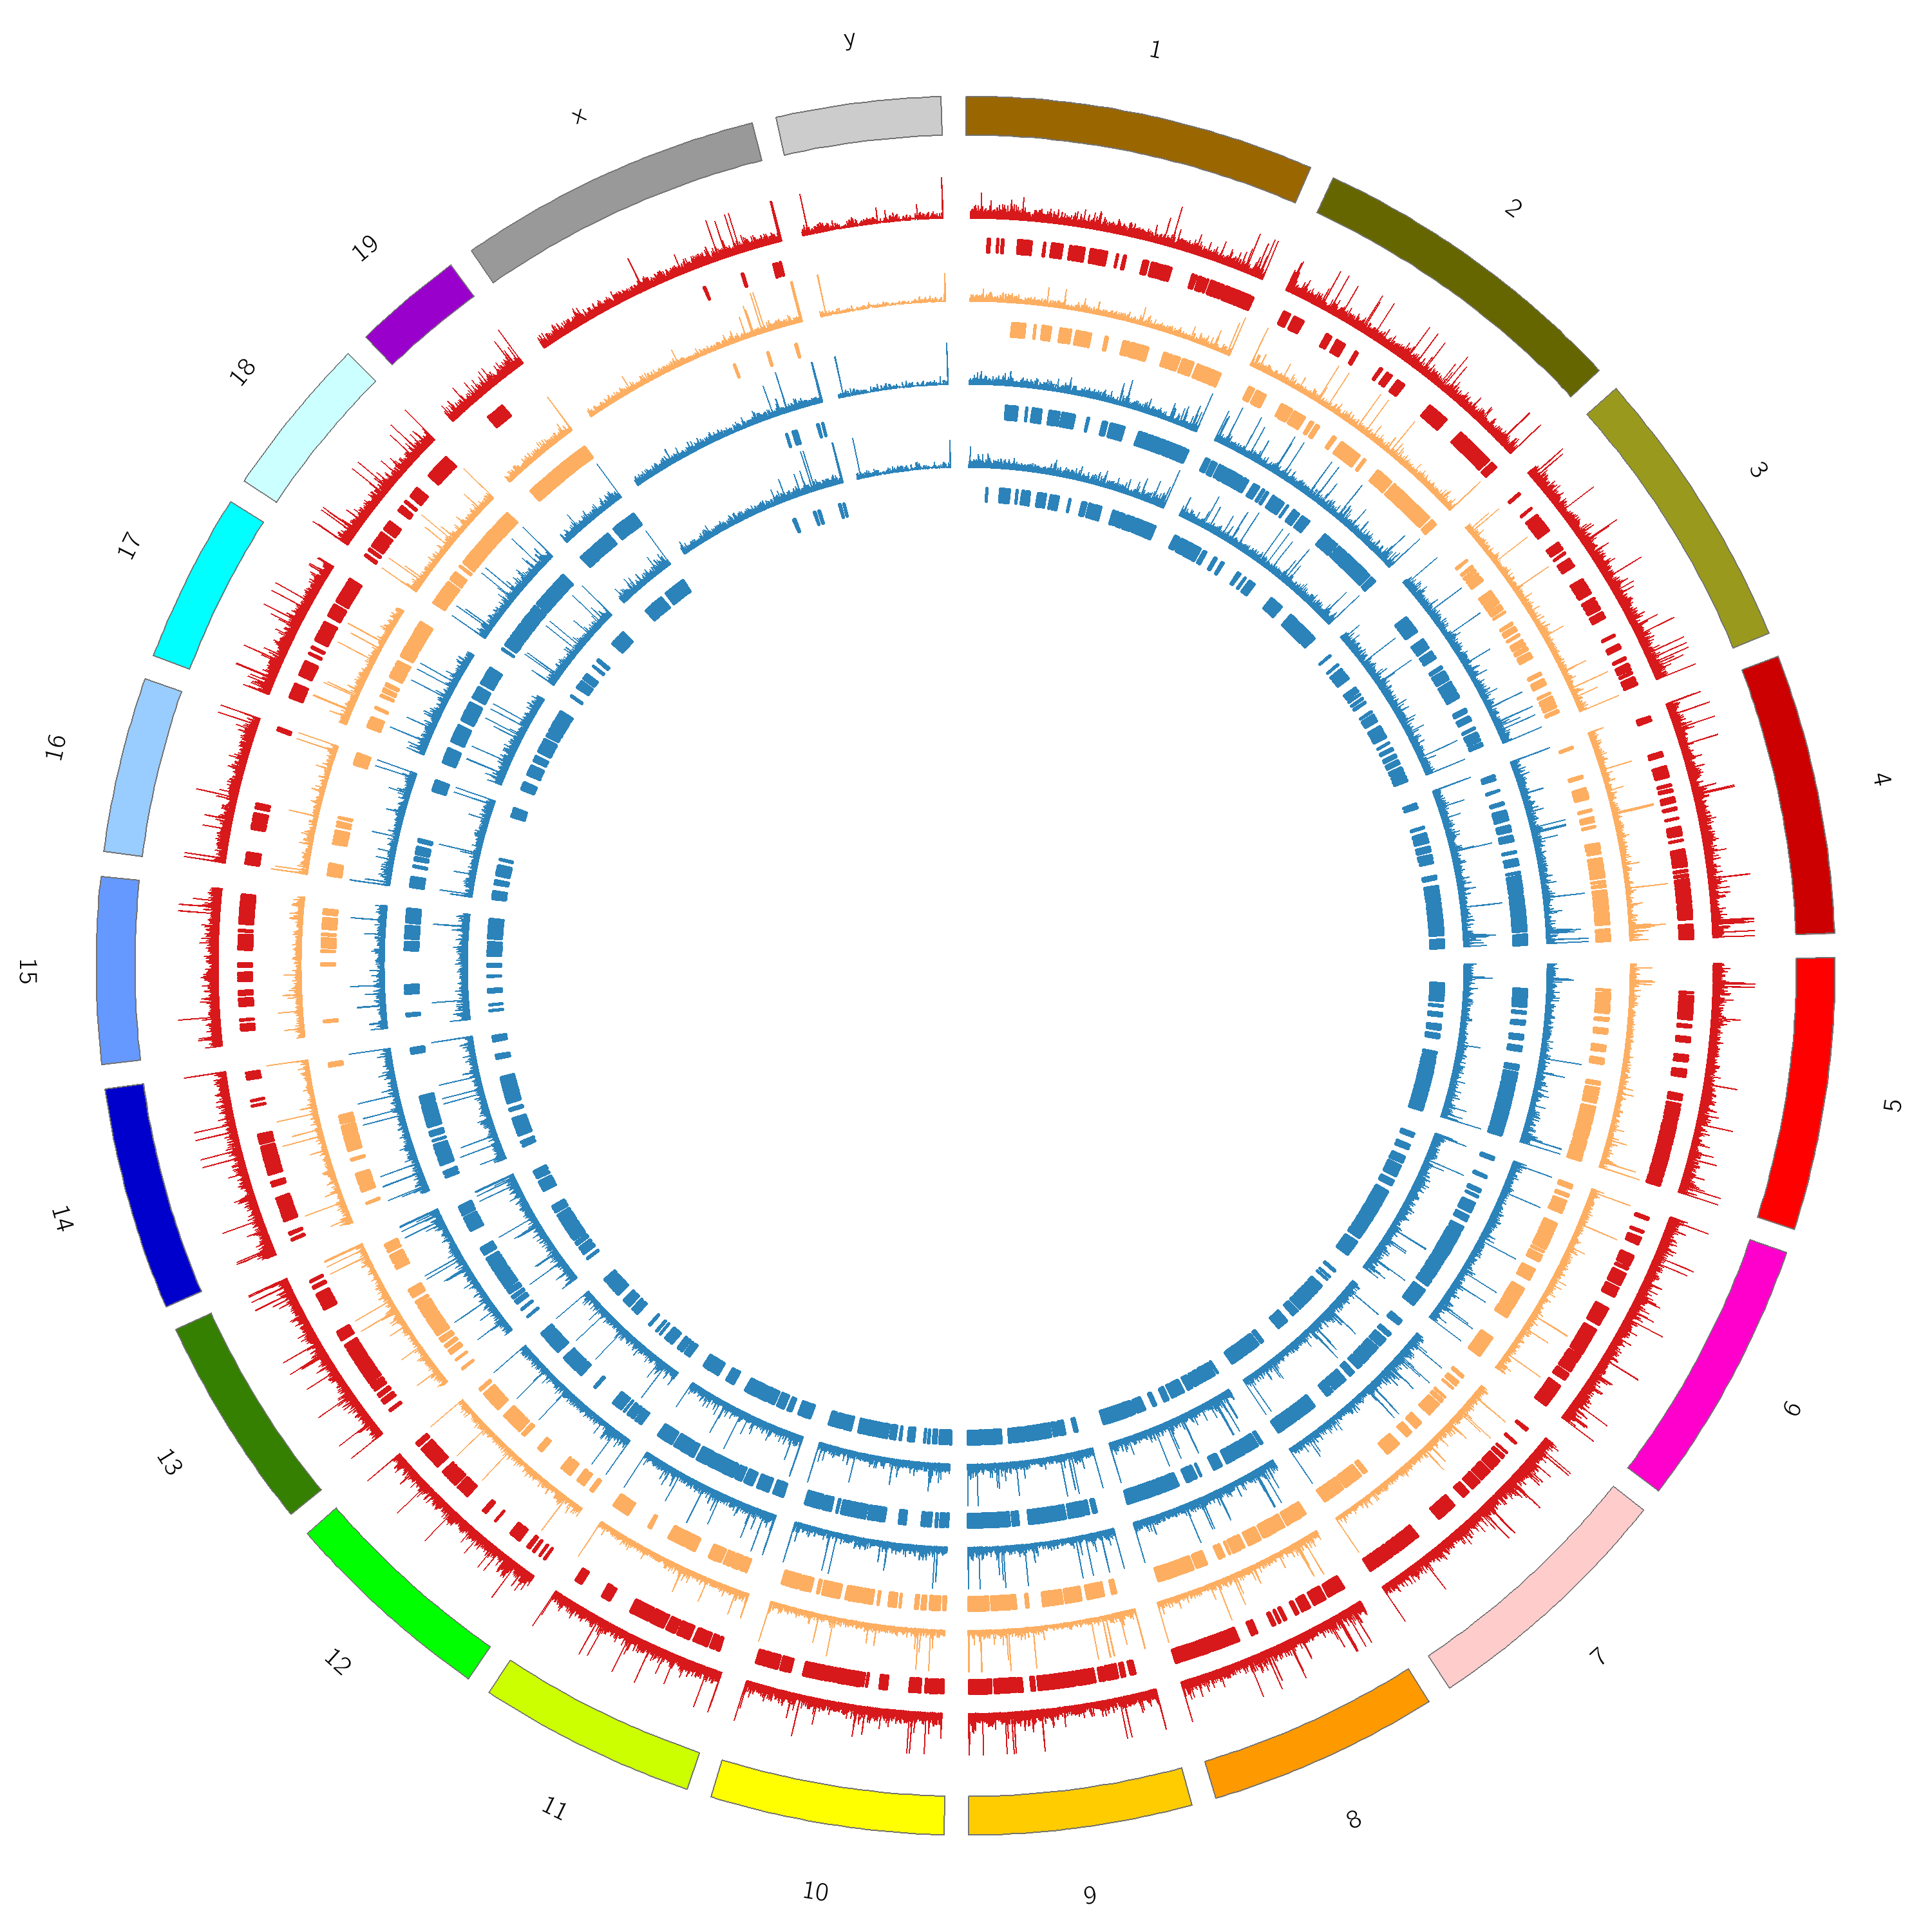
\includegraphics[scale=0.2]{circos2.png}
    \scaption{Répartition du signal normalisé IP-Input pour les différentes librairies (après filtre de la redondance) : le génome de référence mm10 est représenté par le cercle le plus à l'extérieur. Les autres cercles représentent les signaux normalisés des librairies. Les librairies traitées sont en orange pour HD1 et en rouge pour HD2, les librairies contrôles sont bleues.
    L'échelle est fixée arbitrairement à [10:1000]. Les pics EPIC aux FDR non filtrés sont représentés sous le signal leur correspondant. }
    \label{circosTout}
    \end{figure}

\newpage
\section{Manhattan plot pour HDm1 et HDm2}
\begin{figure}[!h]
\centering
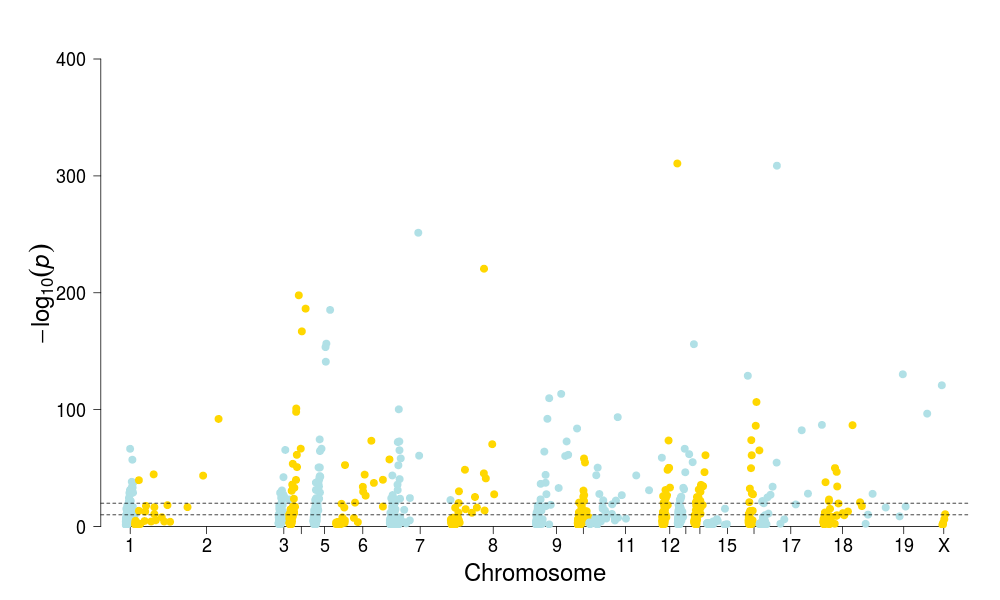
\includegraphics [scale=0.45]{manhattanPlot_lib19EPIC.png}
\scaption{Manhattan plot représentant le FDR en log10 des pics obtenus avec EPIC pour la librairie HDm1. Deux traits horizontaux ont été tracés et correspondent aux FDR à 1 e-10 et 1e-20.}
\label{HDm1M}
\end{figure}


\begin{figure}[!h]
\centering
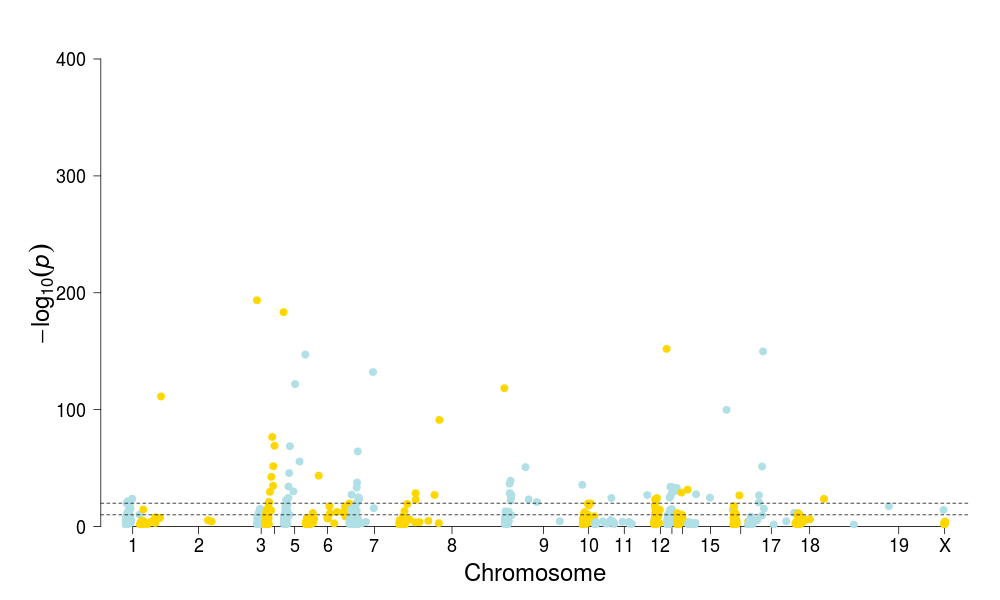
\includegraphics [scale=0.45]{manhattanPlot_lib20EPIC.png}
\scaption{Manhattan plot représentant le FDR en log10 des pics obtenus avec EPIC pour la librairie HDm2. Deux traits horizontaux ont été tracés et correspondent aux FDR à 1 e-10 et 1e-20.}
\label{HDm2M}
\end{figure}





\end{appendices}



\end{document}